\documentclass{report}[11pt]
\usepackage[top=1.0in, bottom=1.0in, left=1.0in, right=1.0in]{geometry}
\usepackage[numbers]{natbib}
\usepackage[pdftex]{graphicx}
\usepackage{booktabs}
\setkeys{Gin}{width=\textwidth}
\usepackage{epstopdf, listings, color, setspace, tocloft, hyperref, cleveref, appendix}
\usepackage[section]{placeins}
\epstopdfsetup{update,prepend}
\graphicspath{{./figures/}}
\epstopdfsetup{suffix=}
\doublespacing
\definecolor{dkgreen}{rgb}{0,0.6,0}
\definecolor{gray}{rgb}{0.5,0.5,0.5}
\definecolor{purple}{rgb}{0.73,0.33,0.83}
% \lstset{
%    language=Matlab,
%   morekeywords={break,case,catch,continue,else,elseif,end,for,function,
%       global,if,otherwise,persistent,return,switch,try,while,ones,
%       squeeze,warning,waitbar,circshift},
%    basicstyle=\small\ttfamily,
%    keywordstyle=\color{blue},
%    commentstyle=\color{dkgreen},
%    stringstyle=\color{purple},
%    frame=leftline,
%    rulecolor=\color{black},
%    numbers=left,
%    numberstyle=\footnotesize,
%    stepnumber=1,
%    numbersep=13pt,
%    backgroundcolor=\color{white},
%    tabsize=2,
%    showspaces=false,
%    showstringspaces=false,
%    breaklines=true
%    }
\lstdefinestyle{codeblock}{
   language=Matlab,
  morekeywords={break,case,catch,continue,else,elseif,end,for,function,
      global,if,otherwise,persistent,return,switch,try,while,ones,
      squeeze,warning,waitbar,circshift},
   basicstyle=\small\ttfamily,
   keywordstyle=\color{blue},
   commentstyle=\color{dkgreen},
   stringstyle=\color{purple},
   frame=leftline,
   rulecolor=\color{black},
   numbers=left,
   numberstyle=\footnotesize,
   stepnumber=1,
   numbersep=13pt,
   backgroundcolor=\color{white},
   tabsize=2,
   showspaces=false,
   showstringspaces=false,
   breaklines=true
   }
\lstdefinestyle{snippet}{
   language=Matlab,
  morekeywords={break,case,catch,continue,else,elseif,end,for,function,
      global,if,otherwise,persistent,return,switch,try,while,ones,
      squeeze,warning,waitbar,circshift},
   basicstyle=\small\ttfamily,
   keywordstyle=\color{blue},
   commentstyle=\color{dkgreen},
   stringstyle=\color{purple},
   rulecolor=\color{black},
   stepnumber=1,
   numbersep=5pt,
   backgroundcolor=\color{white},
   tabsize=2,
   showspaces=false,
   showstringspaces=false,
   breaklines=true,
   xleftmargin=17pt,
   framexleftmargin=17pt,
   framexrightmargin=5pt,
   framexbottommargin=4pt,
   % frame=bottomline
}
\renewcommand{\cftchapdotsep}{\cftdotsep}
\newenvironment{code}
{\begin{list}{}{\setlength{\leftmargin}{1em}}\item\scriptsize\bfseries}
{\end{list}}
\newcommand{\signhere}{\vspace{0.4in}\rule{\linewidth}{0.5mm}\\}
\newcommand{\degree}{\ensuremath{^\circ}}
%%%%%  Put in your title here: %%%%%%
\newcommand{\thesisTitle}{Brain tissue temperature dynamics during functional activity and possibilities for Imaging}
\setcounter{tocdepth}{3}
\setcounter{secnumdepth}{2}
\begin{document}
% Everything is kept in seperate *.tex files.  Use this file to change the orders.
\pagenumbering{roman}
\thispagestyle{empty}
\begin{titlepage}
\begin{center}
\vspace*{\fill}
{ \huge \thesisTitle } \\
\vspace{1.0in}
by \\
\vspace{1.0in}
{ \large \textsc{Greggory H. Rothmeier} } \\
\vspace{2.0in}
A Thesis Submitted in Partial Fulfillment of the Requirements for the Degree of\\
Masters of Science\\
in the College of Arts and Sciences\\
Georgia State University\\
2012\\
\vspace*{\fill}
\end{center}
\end{titlepage}
Copyright
\thispagestyle{empty}
\begin{center}
  \textsc{\thesisTitle} \\
  \vspace{0.5in}
  by \\
  \vspace{0.5in}
  \textsc{Greggory H. Rothmeier} \\
  \vspace{1in}
\end{center}
\begin{flushright}
  \begin{doublespace}
    Committee Chair:~~~~A. G. Unil Perera \\
    Committee:~~~~Mukesh Dhamala \\
                 Brian Thoms \\
                 D. Michael Crenshaw \\
  \end{doublespace}
\end{flushright}
\vspace{0.5in}
\begin{flushleft}
  Electronic Version Approved: \\
  \vspace{0.5in}
  \begin{doublespace}
    Office of Graduate Studies\\
    College of Arts and Sciences\\
    Georgia State University\\
    May 2012\\
  \end{doublespace}
\end{flushleft}
\vspace*{\fill}
\phantomsection
\addcontentsline{toc}{chapter}{Dedication}
\begin{doublespace}
  \begin{center}
    \textbf{Dedication}
  \end{center}
This is dedicated to my parents who made me go to college and to Brooke who inspired me to go to graduate school.  If I wasn't lucky enough to have all of you I would probably be working for Geek Squad.
  
I also want to more specifically dedicate this to my mama.  I miss you and I think about you every day.
\end{doublespace}
\addcontentsline{toc}{chapter}{Acknowledgments}
\begin{doublespace}
  \begin{center}
    \textbf{Acknowledgements}
  \end{center}
  Perera, Dhamala, Brooke, Lab Mates, Dhamala's Lab
\end{doublespace}
\tableofcontents
\clearpage
\addcontentsline{toc}{chapter}{List of Tables}
\listoftables
\clearpage
\addcontentsline{toc}{chapter}{List of Figures}
\listoffigures
\begin{doublespace}
\begin{center}
  \textsc{Awesome title}\\
  \vspace{0.4in}
  A thesis\\
  presented in Partial Fulfilment of Requirements for the Degree of Master of Science in the\\
  College of Arts and Sciences\\
  Georgia State University\\
  2012\\
  by\\
  Greggory Rothmeier\\
  \vspace*{\fill}
  Committee:\\
  \begin{singlespace}
    \signhere
    A. G. Unil Perera, Chair\\
    \signhere
    Mukesh Dhamala, Member\\
    \signhere
    Brian Thoms, Member\\
    \signhere
    D. Michael Crenshaw, Member \\
    \vspace{0.2in}
    April 1, 2012\\
    \rule{\linewidth}{0.5mm}
    Date\\
    \signhere
    Dick Miller\\
    Department Chair\\
    \vspace{0.1in}
  \end{singlespace}
\end{center}
\end{doublespace}
\pagenumbering{arabic}
\setcounter{page}{1}
%%%%%  Chapters  %%%%%%%%%%%%%%
% List of Chapters in the order they need to appear
\chapter{Introduction}

% Why do temperature modeling?
% What level of temperature resolution is needed?
% What temperature resolution is available?
% How can we improve current detectors? (SP)


Since its invention in the 1950's~\citep{carr1954} and later development in the 1970's~\citep{lauterbur1973}, {M}agnetic {R}esonance {I}maging ({MRI}) has allowed physicians and scientists a detailed view within the human body.
  
  % MODELING BOLD
  \section{Models of the fMRI BOLD Response}
  \label{sec:BOLDmodeling}
  
  \begin{figure}[bt]
    \centering
    \vspace{10pt}
    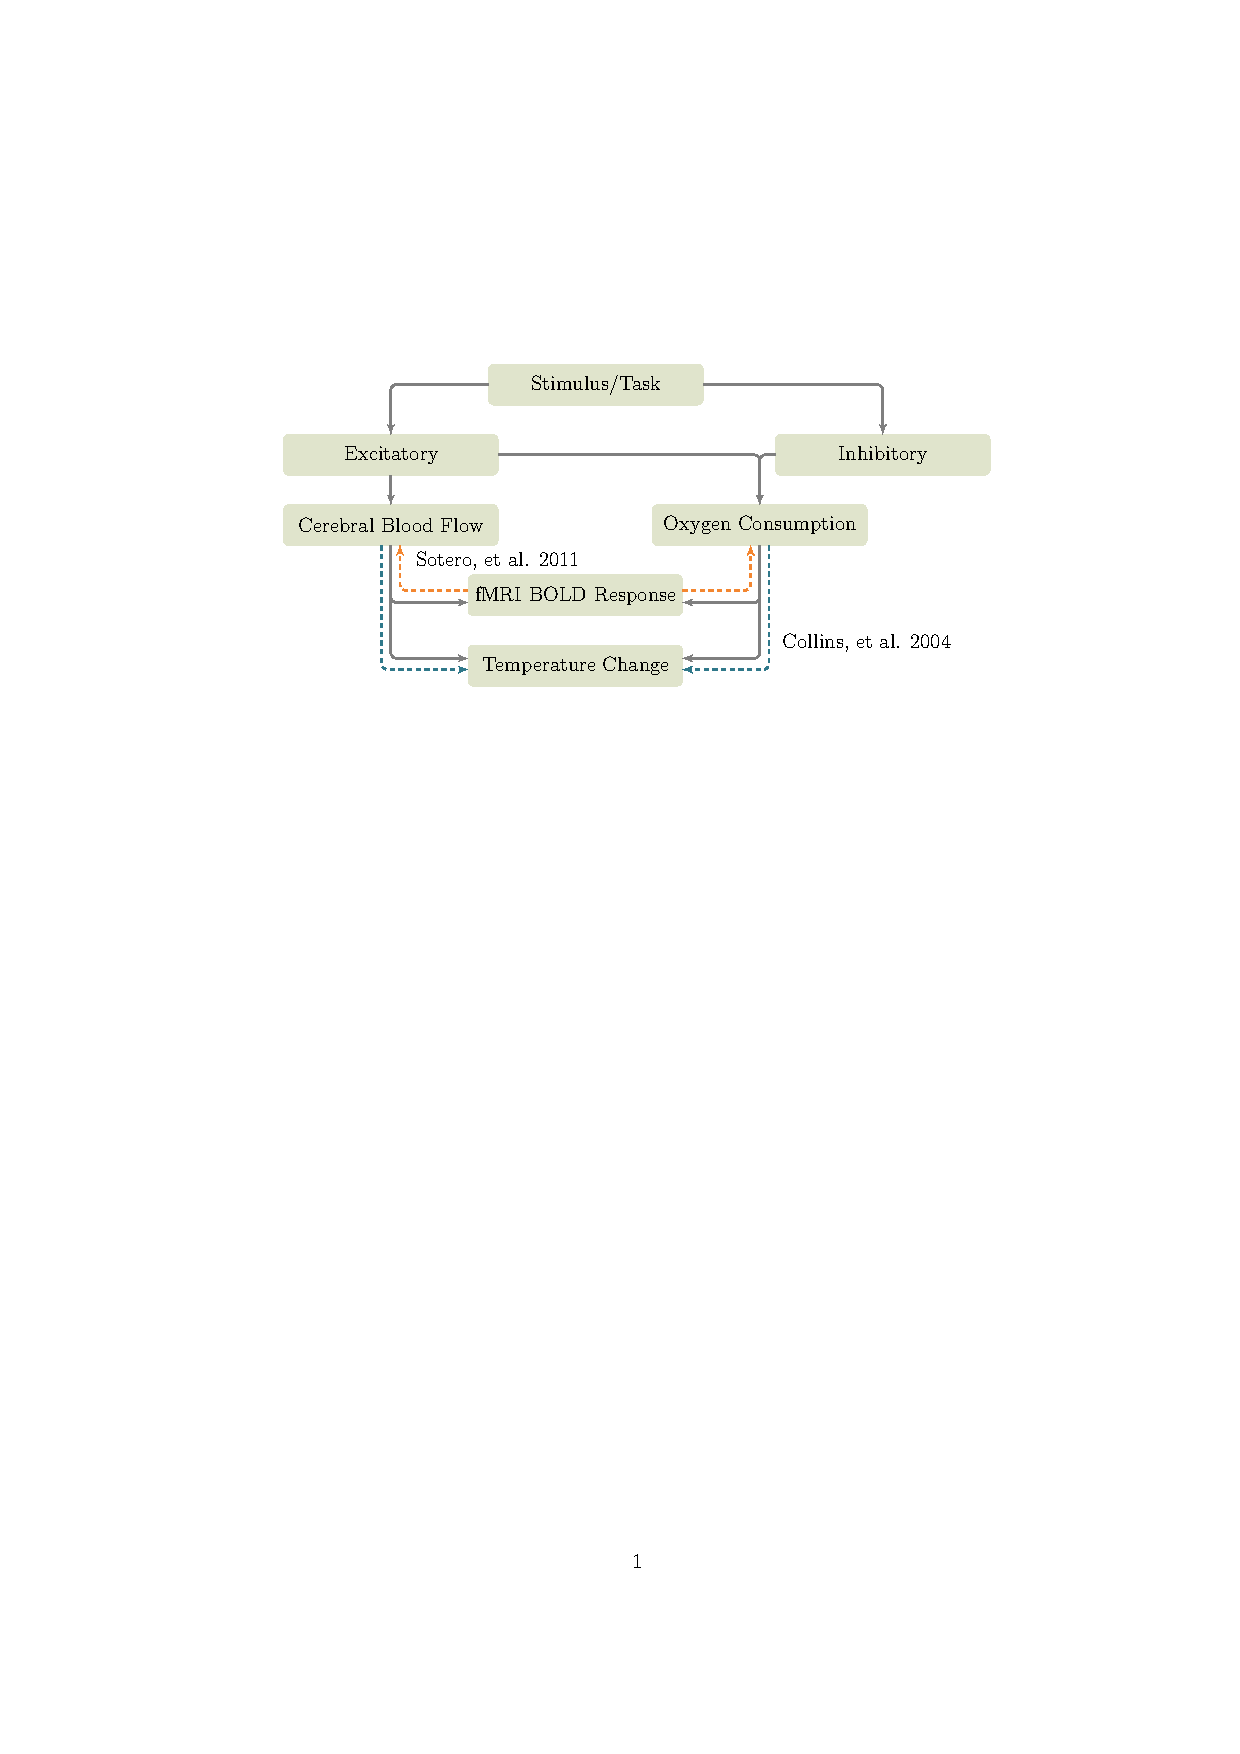
\includegraphics{flowchart}
    % \tikzstyle{block} = [draw=none, fill=beachstorm]
\tikzstyle{line} = [draw, very thick, color=black!50, -stealth']
\tikzstyle{sotero} = [draw, very thick, dashed, color=goldfish, -stealth']
\tikzstyle{collins} = [draw, very thick, dashed, color=aoi, -stealth']
\tikzstyle{citation} = [draw=none, fill=white, minimum height=0.5cm, anchor=north, text width=6.5cm]

\begin{tikzpicture}[node distance=0.7cm, rectangle, text width=4.5cm, text badly centered, rounded corners, minimum height=1cm, anchor=north]
  \node[block](stimulus){Stimulus/Task};
  
  \node[block, below=of stimulus, xshift=-5cm](excitatory){Excitatory Neuronal Activity};
  \node[block, below=of stimulus, xshift= 7cm](inhibitory){Inhibitory Neuronal Activity};
  
  \node[block, below=of excitatory](cbf){Increase in Cerebral Blood Flow (CBF)};
  \node[block, below=of inhibitory, xshift=-3cm](o2){Change in Oxygen Consumption (CMRO$_2$)};
  
  \node[block, below=of cbf, xshift=4.5cm, yshift=-0.5cm](bold){fMRI BOLD Response};
  \node[block, below=of bold](temp){Temperature Change};
  
  \node[citation](sotero1) at (-1.6, -5) {\citet{sotero2011}};
  % \node[citation](sotero1) at (2, -4.5) {Sotero, et. al. 2011};
  % \node[citation](sotero1) at (-4.5, -7.5) {Collins, et. al. 2011};
  \node[citation](sotero1) at (6, -6.5) {\citet{collins}};
  
  \path[line](stimulus.west) -| (excitatory.north);
  \path[line](stimulus.east) -| (inhibitory.north);
  \path[line](excitatory.south) -- (cbf.north);
  \path[line](excitatory.east) -| (o2.north);
  \path[line](inhibitory.west) -| (o2.north);
  
  \path[line](cbf.south) |- ([yshift=-5pt] bold.west);
  \path[line](cbf.south) |- ([yshift= 5pt] temp.west);
  \path[line](o2.south)  |- ([yshift=-5pt] bold.east);
  \path[line](o2.south)  |- ([yshift= 5pt] temp.east);
  
  \path[sotero]([yshift= 5pt] bold) -| ([xshift= 20pt] cbf);
  \path[sotero]([yshift= 5pt] bold) -| ([xshift=-20pt] o2);
  \path[collins]([xshift=-45pt] cbf) |- ([yshift=-5pt] temp);
  \path[collins]([xshift=45pt] o2)  |- ([yshift= -5pt] temp);
\end{tikzpicture}
    \caption[Generation of the fMRI BOLD response and a corresponding temperature change]{\label{fig:flowchart} Generation of the fMRI BOLD response from changes in neuronal activity.  Black arrows indicate a causal relationship while colored dashed-arrows indicate existing models for the relationship.  The orange line ($\color{goldfish}\bullet$) shows the model proposed by~\citet{sotero2011} to calculate cerebral blood flow and metabolism and the blue line ($\color{aoi}\bullet$) shows how the model proposed by~\citet{collins} is used to calculate temperature.}
  \end{figure}
  % Start with Buxton and Friston and build up to how I am calculating the metabolism and blood flow.
  This is just place holder text until I write the introduction (last step).  Hopefully this is sufficient to demonstrate the format.
  
  Lorem ipsum dolor sit amet, consectetur adipiscing elit. Nulla ligula lorem, malesuada non feugiat a, bibendum sit amet leo. Sed in dui lacus. Nullam quam dolor, elementum ac semper vitae, lacinia et dui. Curabitur accumsan urna nec dolor porttitor mollis. Nunc id feugiat tellus. Proin orci arcu, egestas a tincidunt eu, luctus ut ligula. Curabitur at risus non nulla congue facilisis sed eu velit. Morbi eget bibendum sem.

  Cras vel lectus leo. Donec at ante vel eros condimentum dignissim et at libero. Nullam vitae purus at diam semper gravida. Ut venenatis dapibus nulla pretium eleifend. Nam scelerisque dignissim augue, ac suscipit tellus vestibulum vel. Sed rutrum sollicitudin sodales. Pellentesque cursus lobortis neque, id ornare purus laoreet eget. Sed adipiscing sollicitudin convallis. Quisque eu orci sit amet libero mollis tincidunt. Nullam sed consectetur odio. Etiam a molestie orci.

  Pellentesque sed purus odio. Nam pharetra aliquam augue vitae porta. Phasellus malesuada rhoncus tristique. Donec cursus, nibh vel eleifend bibendum, ante massa imperdiet mauris, vel varius dolor libero feugiat nibh. Sed libero sem, bibendum eu cursus sit amet, euismod in dui. Vestibulum massa nisl, accumsan eu cursus nec, pretium blandit lectus. Phasellus vitae ipsum eget tellus consequat molestie vel nec tortor. Curabitur blandit, lectus lacinia consectetur varius, leo metus placerat nisl, ullamcorper egestas nisl nisi in nulla.

  Nunc sit amet mi sed ante dictum luctus eget et augue. Morbi vitae nunc justo. Praesent ac elit lorem. In hac habitasse platea dictumst. Integer pellentesque eros viverra justo scelerisque mollis. Vestibulum tempor tempus velit, et pulvinar odio iaculis ut. Quisque luctus massa sit amet justo ornare nec posuere eros aliquam. Vestibulum luctus pharetra augue, et varius ligula sollicitudin sit amet. Cras mi enim, laoreet quis vulputate ut, pulvinar vel nibh.

  Cras sem justo, ultricies eget sodales eget, bibendum non neque. Pellentesque tempus mi eget massa venenatis id cursus sem aliquet. Nunc venenatis, est at porta faucibus, erat sem ultrices magna, eget tincidunt orci lorem vitae nisl. Sed sem velit, fermentum in hendrerit eu, tempor fermentum arcu. Nullam id nunc vel purus aliquet faucibus. Donec ullamcorper odio ac purus tristique mollis. Class aptent taciti sociosqu ad litora torquent per conubia nostra, per inceptos himenaeos. Pellentesque eget elit in orci iaculis congue. Suspendisse sit amet nisl a velit tempus pretium. Suspendisse quis vulputate nunc. Phasellus quis elit sit amet arcu faucibus adipiscing. Vestibulum faucibus enim ut libero venenatis ac facilisis dolor ultrices.
\chapter{Calculating Temperature Changes using the fMRI BOLD Response}

\section{Background}
  % What does the BOLD response tell us?
  % What gives rise to the fMRI BOLD response?
  % \subsection{Generation of the {B}lood {O}xygen {L}evel {D}ependent ({BOLD}) Response}
  
  Since its invention in the 1950's~\citep{carr1954} and later development in the 1970's~\citep{lauterbur1973}, {M}agnetic {R}esonance {I}maging ({MRI}) has allowed physicians and scientists a detailed view within the human body.
    \begin{figure}[bt]
      \centering
      \vspace{10pt}
      % 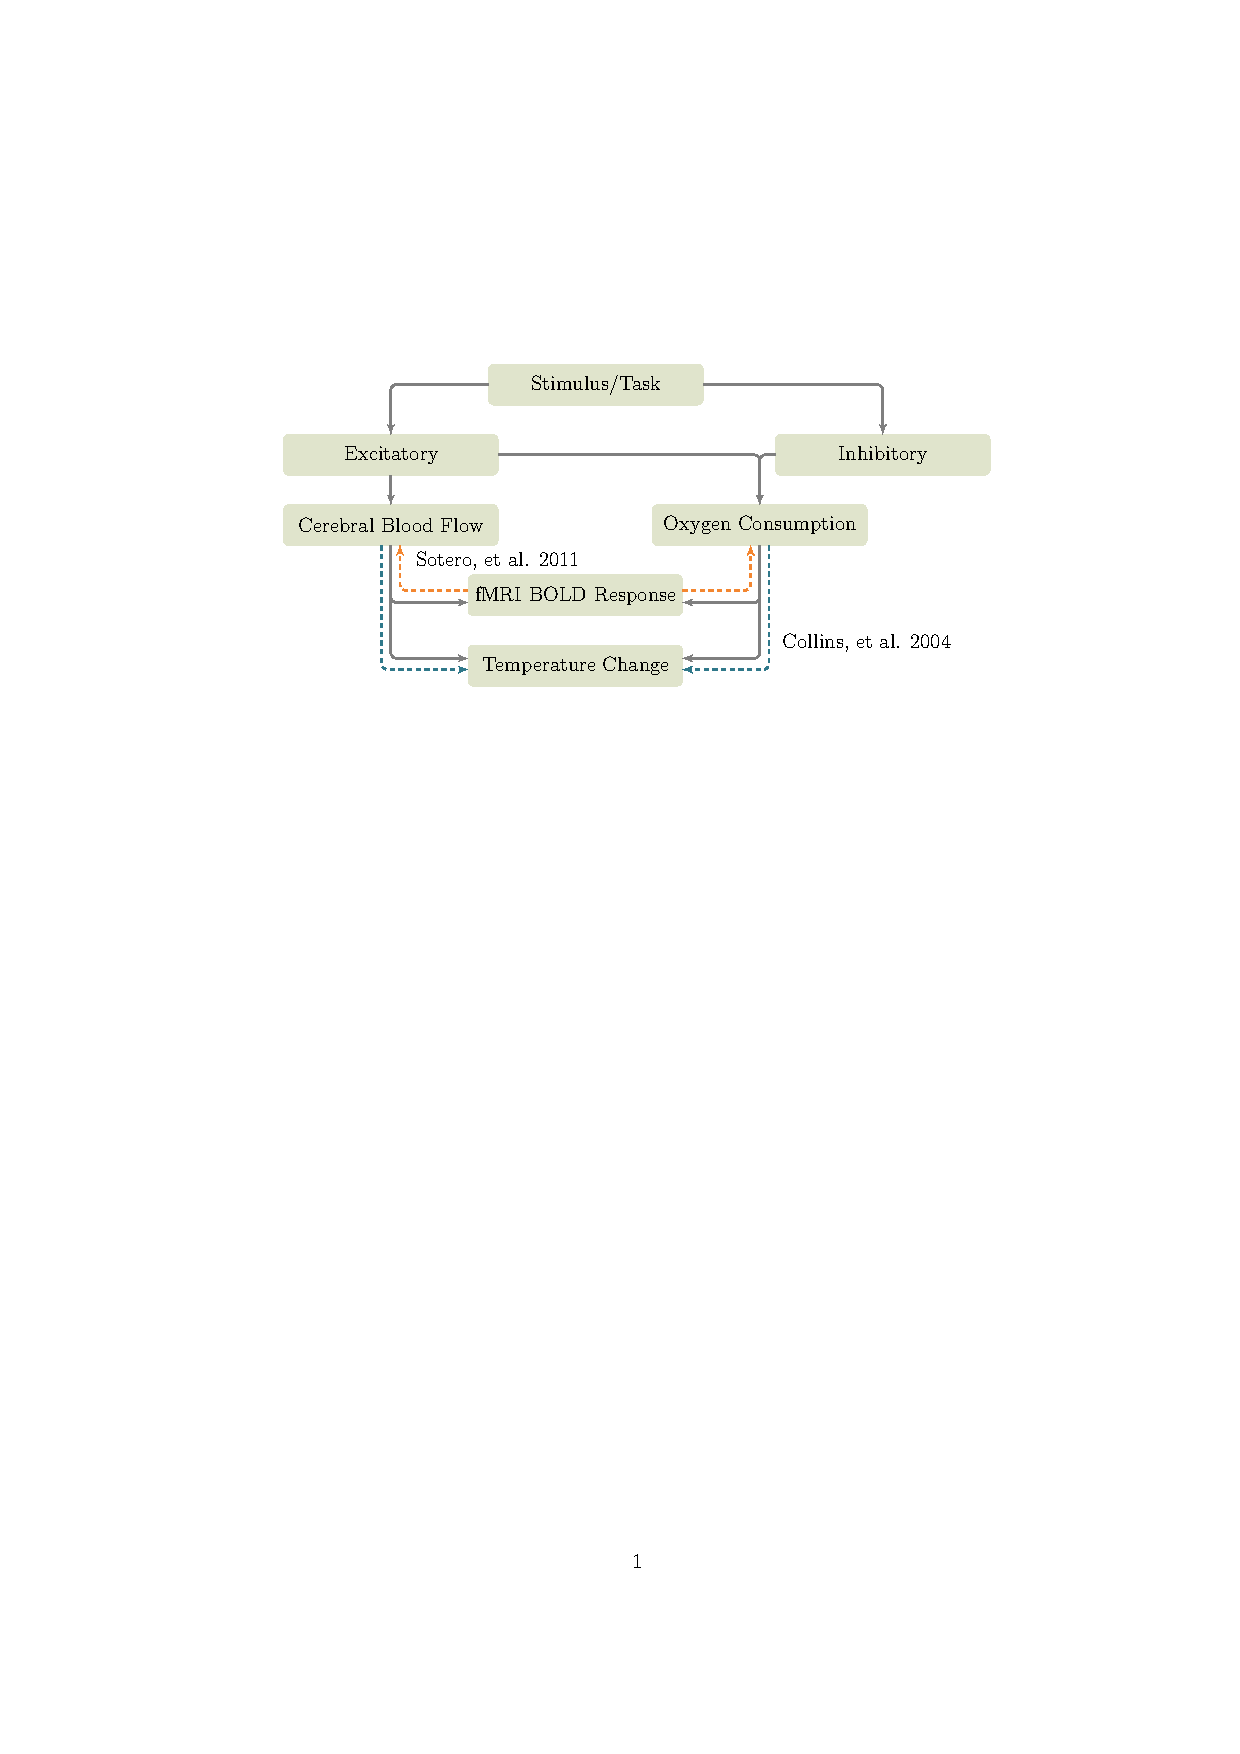
\includegraphics{flowchart}
      \tikzstyle{block} = [draw=none, fill=beachstorm]
\tikzstyle{line} = [draw, very thick, color=black!50, -stealth']
\tikzstyle{sotero} = [draw, very thick, dashed, color=goldfish, -stealth']
\tikzstyle{collins} = [draw, very thick, dashed, color=aoi, -stealth']
\tikzstyle{citation} = [draw=none, fill=white, minimum height=0.5cm, anchor=north, text width=6.5cm]

\begin{tikzpicture}[node distance=0.7cm, rectangle, text width=4.5cm, text badly centered, rounded corners, minimum height=1cm, anchor=north]
  \node[block](stimulus){Stimulus/Task};
  
  \node[block, below=of stimulus, xshift=-5cm](excitatory){Excitatory Neuronal Activity};
  \node[block, below=of stimulus, xshift= 7cm](inhibitory){Inhibitory Neuronal Activity};
  
  \node[block, below=of excitatory](cbf){Increase in Cerebral Blood Flow (CBF)};
  \node[block, below=of inhibitory, xshift=-3cm](o2){Change in Oxygen Consumption (CMRO$_2$)};
  
  \node[block, below=of cbf, xshift=4.5cm, yshift=-0.5cm](bold){fMRI BOLD Response};
  \node[block, below=of bold](temp){Temperature Change};
  
  \node[citation](sotero1) at (-1.6, -5) {\citet{sotero2011}};
  % \node[citation](sotero1) at (2, -4.5) {Sotero, et. al. 2011};
  % \node[citation](sotero1) at (-4.5, -7.5) {Collins, et. al. 2011};
  \node[citation](sotero1) at (6, -6.5) {\citet{collins}};
  
  \path[line](stimulus.west) -| (excitatory.north);
  \path[line](stimulus.east) -| (inhibitory.north);
  \path[line](excitatory.south) -- (cbf.north);
  \path[line](excitatory.east) -| (o2.north);
  \path[line](inhibitory.west) -| (o2.north);
  
  \path[line](cbf.south) |- ([yshift=-5pt] bold.west);
  \path[line](cbf.south) |- ([yshift= 5pt] temp.west);
  \path[line](o2.south)  |- ([yshift=-5pt] bold.east);
  \path[line](o2.south)  |- ([yshift= 5pt] temp.east);
  
  \path[sotero]([yshift= 5pt] bold) -| ([xshift= 20pt] cbf);
  \path[sotero]([yshift= 5pt] bold) -| ([xshift=-20pt] o2);
  \path[collins]([xshift=-45pt] cbf) |- ([yshift=-5pt] temp);
  \path[collins]([xshift=45pt] o2)  |- ([yshift= -5pt] temp);
\end{tikzpicture}
      \caption[Generation of the fMRI BOLD response and a corresponding temperature change]{\label{fig:flowchart} Generation of the fMRI BOLD response from changes in neuronal activity.  Black arrows indicate a causal relationship while colored dashed-arrows indicate existing models for the relationship.  The orange line ($\color{goldfish}\bullet$) shows the model proposed by~\citet{sotero2011} to calculate cerebral blood flow and metabolism and the blue line ($\color{aoi}\bullet$) shows how the model proposed by~\citet{collins} is used to calculate temperature.}
    \end{figure}
    
  \subsection{\label{ss:previousmodels} Previously Proposed Temperature Models}
  Current efforts to model temperature changes be can categorized into two classes.  The first class approaches the problem by considering a single voxel deep within the brain (single-voxel approach) while the second approach considers the brain and head as an entire system (multi-voxel approach).  Each of these methods has their own pros and cons which will be discussed below.
    \subsubsection{Single-Voxel Approach}
    A single-voxel model of temperature was first proposed by SOMEONE, but has been refined over the past HOWLONG years CITEABUNCH to include more terms.  Although different approaches consider different contributions to the temperature change, they all narrow the problem down to a single voxel which is usually 2mm x 2mm x 2mm.  By simplifying the model, the heat equation can be simplified and the calculation is much easier to undertake.  However, since the brain is not homogenous, the values used for parameters such as heat production and thermal conductivity are taken from an average of the tissues.  As a result, this reduces the possible accuracy of such a model when applied to a subject.
    The most recently published iteration of a single-voxel model was published by~\citet{sotero2011}.  The basis of this model is a modification of the Penne's Bioheat Equation~\citep{pennes, sotero2011}.
    %%%%%%%  Bio-heat Equation %%%%%%%%%%%%
    \begin{equation}
      \label{eq:bioheat}
      C_t \frac{dT(t)}{dt} = (\Delta H^{\circ}-\Delta H_{b}) CMRO_{2}\mid_{0} m(t) - \rho_{b} C_{b} CBF\mid_{0} f(t) (T(t) - T_{a}) - \frac{C_{t}}{\tau} (T(t)-T_{0})
    \end{equation}
    where BLA BLA BLA.  
    One advantage of using~\cref{eq:bioheat} is that the resting state temperature can be analytically determined by substituting $\frac{dT(t)}{dt} = 0$~\citep{sotero2011}.
    %%%%%%%  Resting state temperature %%%%%
    \begin{equation}
      \label{eq:restingtemperature}
      T_{0} = T_{a} + \frac{(\Delta H \mid^{\circ} - \Delta H_{b}) CMRO_{2}\mid_{0}}{\rho_{B} C_{B} CBF\mid_{0}}
    \end{equation}
    If the values provided in~\cref{tbl:soteroparams} are substitued into~\cref{eq:restingtemperature}, a resting temperature of 37.3057\degree C is found.  Since the resting temperature is always greater than the arterial blood temperature, it limits the ability of the model to account for all experimental results. 
    
    While~\cref{eq:bioheat} is appears complicated, conceptually the equation can be easily understood.
    %%%%%%%  Explanation %%%%%%%%%%%%%%%%%%%
    \begin{equation}    
      \label{eq:soteroexplaiend}
      change\ in\ temperature\ =\ heat\ generated\ by\ metabolism\ -\ heat\ lost\ to\ convection\ -\ heat\ lost\ to\ conduction
    \end{equation}
    The system is a balance between heat generation (metabolism) and heat transfer (conduction and convection).  The direction of heat transfer by convection is determined by the difference between the voxel temperature and the arterial blood temperature ($T(t) - T_a$).  Similarly, the direction of heat transfer by conduction is determined by the difference between the voxel temperature and the temperature of the surrounding tissue ($T(t) - T_0$).  Since $T_a$ is less than $T(0)$, an increase in blood flow ($f(t)$) will remove heat from the voxel thereby decreasing the temperature.  Conversely, an increase in metabolism ($m(t)$) without a corresponding change in blood flow, will result in tissue warming.  
    
    
    
    %%%%  Table of values used in Sotero, 2011  %%%%%
    \begin{table*}[bt]
      \caption[Parameters used in the single-voxel approximation]{\label{tbl:soteroparams} Parameters used to solve the single-voxel Penne's Bioheat Equation.  (modified from~\citet{sotero2011})}
        \begin{tabular*}{\linewidth}{lp{10cm}p{4cm}}
          \toprule
          Parameter & Meaning & Value \\
          \midrule
          T$_{a}$ & Arterial blood temperature & 37\degree C \\
          $C_{tissue}$ & Tissue Heat Capacity & 3.664 J/(gK) \\
          $\Delta H^{\circ}$ & Enthalpy released by oxidation of glucose & $4.7 10^{5}$ J \\
          $\Delta H_{b}$ & Enthalpy used to release O$_{2}$ from hemoglobin & $2.8 10^{4}$ J \\
          CMRO$_{2}\mid_{0}$ & Cerebral metabolic rate of O$_{2}$ consumption at rest & $0.0263 10^{-6}$ mol/(gs) \\
          CBF$\mid_{0}$ & Cerebral blood flow at rest & 0.0093 cm\textsuperscript{3}/(gs) \\
          $\rho_{b}$ & Blood density & 1.05 g/cm\textsuperscript{3} \\
          C$_{B}$ & Blood heat capacity & 3.894 J/(gK) \\
          $\tau$ & Time constant for conductive heat loss from the ROI to the surrounding tissue & 190.52 s \\
          a, b, c & Parameters of the gamma function fitted from E(f) vs. f & 0.4492, 0.2216, -0.9872 \\
          A & Maximum BOLD signal change & 0.22 \\
          $\alpha$ & Steady state flow-volume relation & 0.4 \\
          $\beta$ & Field-strength dependent parameter & 1.5 \\
          \midrule
          Variable & Meaning & \\
          \midrule
          m(t) & CMRO$_2$ normalized to baseline & \\
          f(t) & CBF normalized to baseline & \\
          T(t) & Temperature & \\
          W(t) & Lambert W Function & \\
          $\frac{\Delta S(t)}{S_0}$ & Change in BOLD signal normalized to rest & \\
          \bottomrule
        \end{tabular*}
    \end{table*}
    
    
    \subsubsection{\label{sss:multivoxel}Multi-Voxel Approach}
  

% MODELING BOLD
\section{Modeling the BOLD Response}
\label{sec:modelingBOLD}
% Start with Buxton and Friston and build up to how I am calculating the metabolism and blood flow.


% MODELING TEMPERATURE
\section{Modeling Temperature}
% THE APPROACH
  \subsection{The Approach}
  \label{sec:theapproach}
  The fundamental difference between our temperature modeling approach and the single-voxel models discussed in~\cref{ss:previousmodels} is that we consider the entire head. The Pennes bioheat equation (\cref{eq:bioheat}) \citep{pennes,sotero2011} includes three terms. The first and second terms describe heat generation by metabolism and heat exchange by convection to blood flow.  On shorter time scales, these two terms dominate and are sufficient for determining the temperature change; however, the third term becomes important on longer time scales.
  
  The third term describes the heat exchanged by conduction to surrounding tissues.  This is a comparatively slow process, but on larger time scales determines the resting state temperature.  When calculating the temperature change, it is important to first have an accurate resting state temperature.  By considering the entire head, out model is able to accurately determine a resting state temperature for each voxel, enabling far more accurate temperature calculations than what is capable with single-voxel approaches.  \Cref{fig:procedureflowchart} gives a schematic of the temperature calculation procedure.
  
  At the heart of our method is a three-dimensional implementation of the Pennes bioheat equation
    \begin{equation} 
    \label{eq:3dbioheat} 
    	\rho c \frac{dT}{dt} = k \nabla^{2}T-\rho_{blood}f(t)wc_{blood}(T-T_{blood})+m(t)Q_{m} 
    \end{equation}
  where $\rho$ is the tissue density, $c$ is the specific heat of the voxel, $k$ is the thermal conductivity, $\rho_{blood}$ is the blood density, $w$ is perfusion by blood, $c_{blood}$ is the specific heat of blood, $T_{blood}$ is the arterial blood temperature, and $Q_{m}$ is the baseline metabolic heat production. $f(t)$ and $m(t)$ are the time-dependent changes in blood flow and metabolism. These two factors determine the short-term change in temperature and are calculated from the fMRI BOLD response.
  \begin{figure}[tb]
    \caption[Procedure used to calculate temperature change]{\label{fig:procedureflowchart} The procedure used to calculate temperature from BOLD data.  Orange blocks ($\color{goldfish}\bullet$) represent data, the sandy-colored block ($\color{beachstorm}\bullet$) is a step done using SPM8 and the teal blocks ($\color{aoi}\bullet$) are steps done using a function provided within temptools (\cref{appendix:code}).}
    \vspace{10pt}
    \centering
    \tikzstyle{data} = [draw=none, fill=goldfish]
\tikzstyle{temptools} = [draw=none, fill=aoi]
\tikzstyle{spm} = [draw=none, fill=beachstorm]
\tikzstyle{params} = [draw=none, fill=pondwater]
\tikzstyle{line} = [draw, very thick, color=black!50, -stealth']

\begin{tikzpicture}[node distance=0.7cm, rectangle, text width=4.5cm, text badly centered, rounded corners, minimum height=1cm, anchor=north]     
  % Left column
    \node[data](fmridata){fMRI BOLD Data};
    \node[temptools, below=of fmridata](calcrest){Calculate resting state (avg\_NII\_rest)};
    \node[temptools, below=of calcrest](normalize){Normalize the data to resting state (avg\_NII\_normalize)};
    \node[temptools, below=of normalize](boldtomf){Calculate the change in metabolism and blood flow (BOLDtoMF)\\Details given in \cref{sec:calcmf}};
    % middle column
    \node[data, right=of fmridata](t1contrast){T1 contrast image};
    \node[spm, below=of t1contrast](segment){Segment image (SPM8)};
    \node[temptools, right=of boldtomf](buildhead){Build head matrix (ImportSegmentedT1)\\Details given in \cref{sec:prephead}};
    % right column
    \node[temptools, right=of buildhead](calcequil){Calculate equilibrium temperature (tempCalcEquilibrium)\\Details given in \cref{sec:calcequilT}};
    \node[params, above=of calcequil, xshift=-2cm](tissueparams){Tissue-specific parameters (given in \cref{tbl:tissues})};
    % bottom
    \node[temptools, below=of buildhead, text width=8cm](calctemp){Find temperature change during activity (tempCalcDynMF)\\Details given in \cref{sec:calcT}};
  
  \path[line](fmridata) -- (calcrest);
  \path[line](calcrest) -- (normalize);
  \path[line](normalize) -- (boldtomf);
  \path[line](t1contrast) -- (segment);
  \path[line](segment) -- (buildhead);
  \path[line](buildhead) -- (calcequil);
  \path[line](boldtomf) |- (calctemp);
  \path[line](buildhead) -- (calctemp);
  \path[line](calcequil) |- (calctemp); 
  \path[line](tissueparams) -| (buildhead);
\end{tikzpicture}
  \end{figure}
  
  % SETUP AND FILE PROCESSING
    \subsubsection{Preparing the model of the head}
    \begin{figure}[tb] 
      \centering \hspace*{20px} 
    	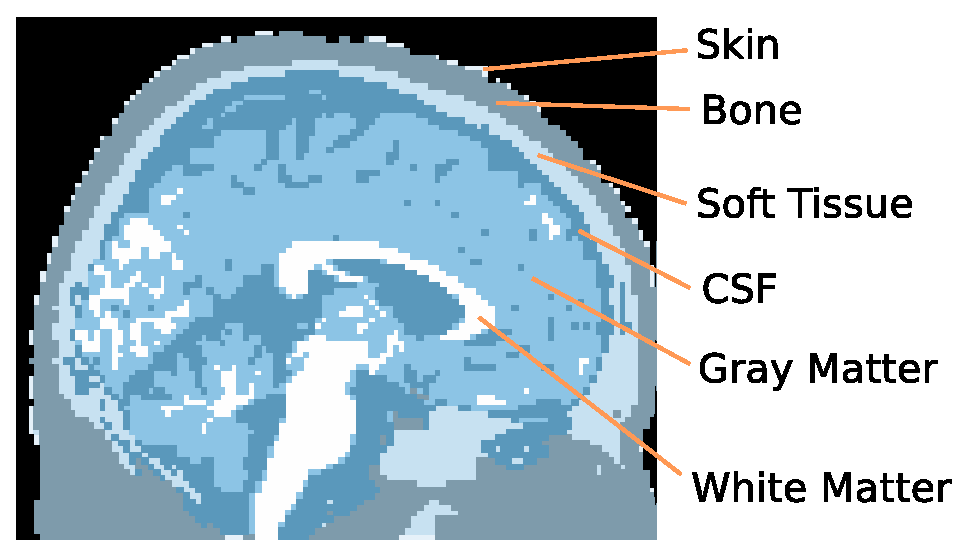
\includegraphics{segmented-head} 
    	\caption{\label{fig:segmented} Slice of the segmented head. Each color represents a different tissue type.} 
    \end{figure}
    \begin{table*}[tb] 
      \caption[Tissue-specific parameters]{\label{tbl:tissues} Tissue-specific parameters used to calculate the temperature change (from~\citet{collins}).} 
      \vspace{10pt}
    		\begin{tabular*}{\linewidth}{llllll} 
    		  \toprule
    		  Tissue & $f_0, 100*ml g^{-1} min^{-1}$ & $\rho, kg/m^{3}$ & $c, J kg^{-1}*\degree C^{-1}$ & $k, W m^{-1}*\degree C^{-1}$ & $Q_{m}, W/m^{3}$ \\
    		  \midrule
    			Bone & 3 & 1,080 & 2,110 & 0.65 & 26.1 \\
    			Cerebrospinal Fluid & 0 & 1,007 & 3,800 & 0.50 & 0 \\
    			Gray Matter & 67.1 & 1,035.5 & 3,680 & 0.565 & 15,575 \\
    			White Matter & 23.7 & 1,027.4 & 3,600 & 0.503 & 5,192 \\
    			Muscle & 3.8 & 1,041 & 3,720 & 0.4975 & 687 \\
    			Skin & 12 & 1,100 & 3,150 & 0.342 & 1,100 \\
    			\bottomrule
    		\end{tabular*}
    \end{table*}
  In order to begin the temperature calculating procedure, a model of the head must first be created.  Using SPM8 (\url{http://www.fil.ion.ucl.ac.uk/spm/}), we segmented a T1 contrast image of the head into five different tissue types: bone, cerebral spinal fluid, gray matter, white matter and soft tissue.  It was assumed that soft tissue voxels that are incontact with air are more appropriately labeled as skin, so in total we are left with a model of the head separated in to six tissue types (\cref{fig:segmented}).  The advantage this has is that we are able to use tissue specific parameters when doing the calculations, thereby improving the accuracy of the results.  The parameters used are available in~\cref{tbl:tissues}.  The code used to create the head matrix is discussed in~\cref{sec:headmatrix}.

  
  % CALC EQUIL T
    \subsubsection{Calculating the equilibrium temperature}
  The first step in calculating the temperature change is to first know what the resting state temperature is for each voxel within the head. Our approach was to have the initial temperature for all tissue voxels to be equal to 37\degree C and air voxels are kept at 24\degree C.  The starting temperature of the tissue doesn't affect the final resting state temperature; however, starting off at drastically different values could greatly increase the calculating time required before the temperature stabilizes. The finite difference implementation of the Pennes bioheat equation (\cref{eq:3dbioheat}) is used to update the temperature.  The temperature is updated until the temperature for every voxel has stabilized ($\frac{dT}{dt} < 10^{-6}$ \degree C/s).  Since temperature changes due to changes in neuronal activity are typically greater than $10^{-2}$ \degree C, a change in temperature less than $10^{-6}$ \degree C/s is sufficiently small that transient temperature changes are negligible and temperature can be considered stabilized.  The code used to calculate the equilibrium temperature is detailed in~\cref{sec:findequil}.
  
  % CALC M AND F
    \subsubsection{Calculating Metabolism and Blood Flow Changes from fMRI BOLD}
    \label{sss:calcmf}
    This is the critical step where we use fMRI BOLD data to calculate the normalized change in metabolism and blood flow.  The method used~\cite{sotero2011} is an assemblage of a couple other works [CITATION NEEDED]. The input data is a folder containing a BOLD dataset taken at equal time intervals.  The first step in processing the data for temperature calculations is to determine a resting state.  The resting state is calculated by taking the element-wise mean of the data when the subject is at rest (i.e. the first and last 20 seconds).  This results in one data set where each voxel is a mean of all of the voxels at the location over time ($S_0$).  In order to calculate the metabolism and blood flow, the BOLD dataset needs to be normalized to this resting state ($S(t)/S_0$).  This can then be used to calculate a BOLD-dependent variable, $y(t)$
    \begin{equation}
      \label{eq:y} 
    	y(t)=-\frac{b \beta}{\alpha+\beta c} \left[\frac{(A-\frac{S(t)}{S_{0}}-1)}{A a^{\beta}}\right]^{\left(\frac{1}{\alpha+\beta c}\right)} 
    \end{equation}
  where A is the maximum change in BOLD that can occur; $\alpha$ comes from a steady state flow-volume relation; $\beta$ is a field-strength dependent parameter; and a, b, and c are parameters of the gamma function fitted from E(f) vs. f (values provided in~\cref{tbl:soteroparams}) \cite{sotero2011}. With $y(t)$,  the change in blood flow can be calculated as follows
    \begin{equation}
      \label{eq:f}
      f(t)=\frac{\alpha+\beta c}{b \beta}W(y(t))
    \end{equation}
  where W(y(t)) is the Lambert-W function of y(t). From $f(t)$, the change in metabolism $m(t)$ can be determined
    \begin{equation}
      \label{eq:m} 
      m(t)=af^{c+1}(t)e^{-bf(t)}.
    \end{equation}
  The implementation of these functions is available in~\cref{sec:fmriprocessing}. 
  % CALC CHANGE IN T
    \subsubsection{Calculating the change in temperature in the active brain}
% RESULTS
  \subsection{Results}
  \label{sec:results}
    \subsubsection{Using Theoretical BOLD Data}
    \FloatBarrier
    \begin{figure}[p] 
    	\begin{center}
    		\begin{tabularx}{\textwidth}{cc}
    			\raisebox{20px}{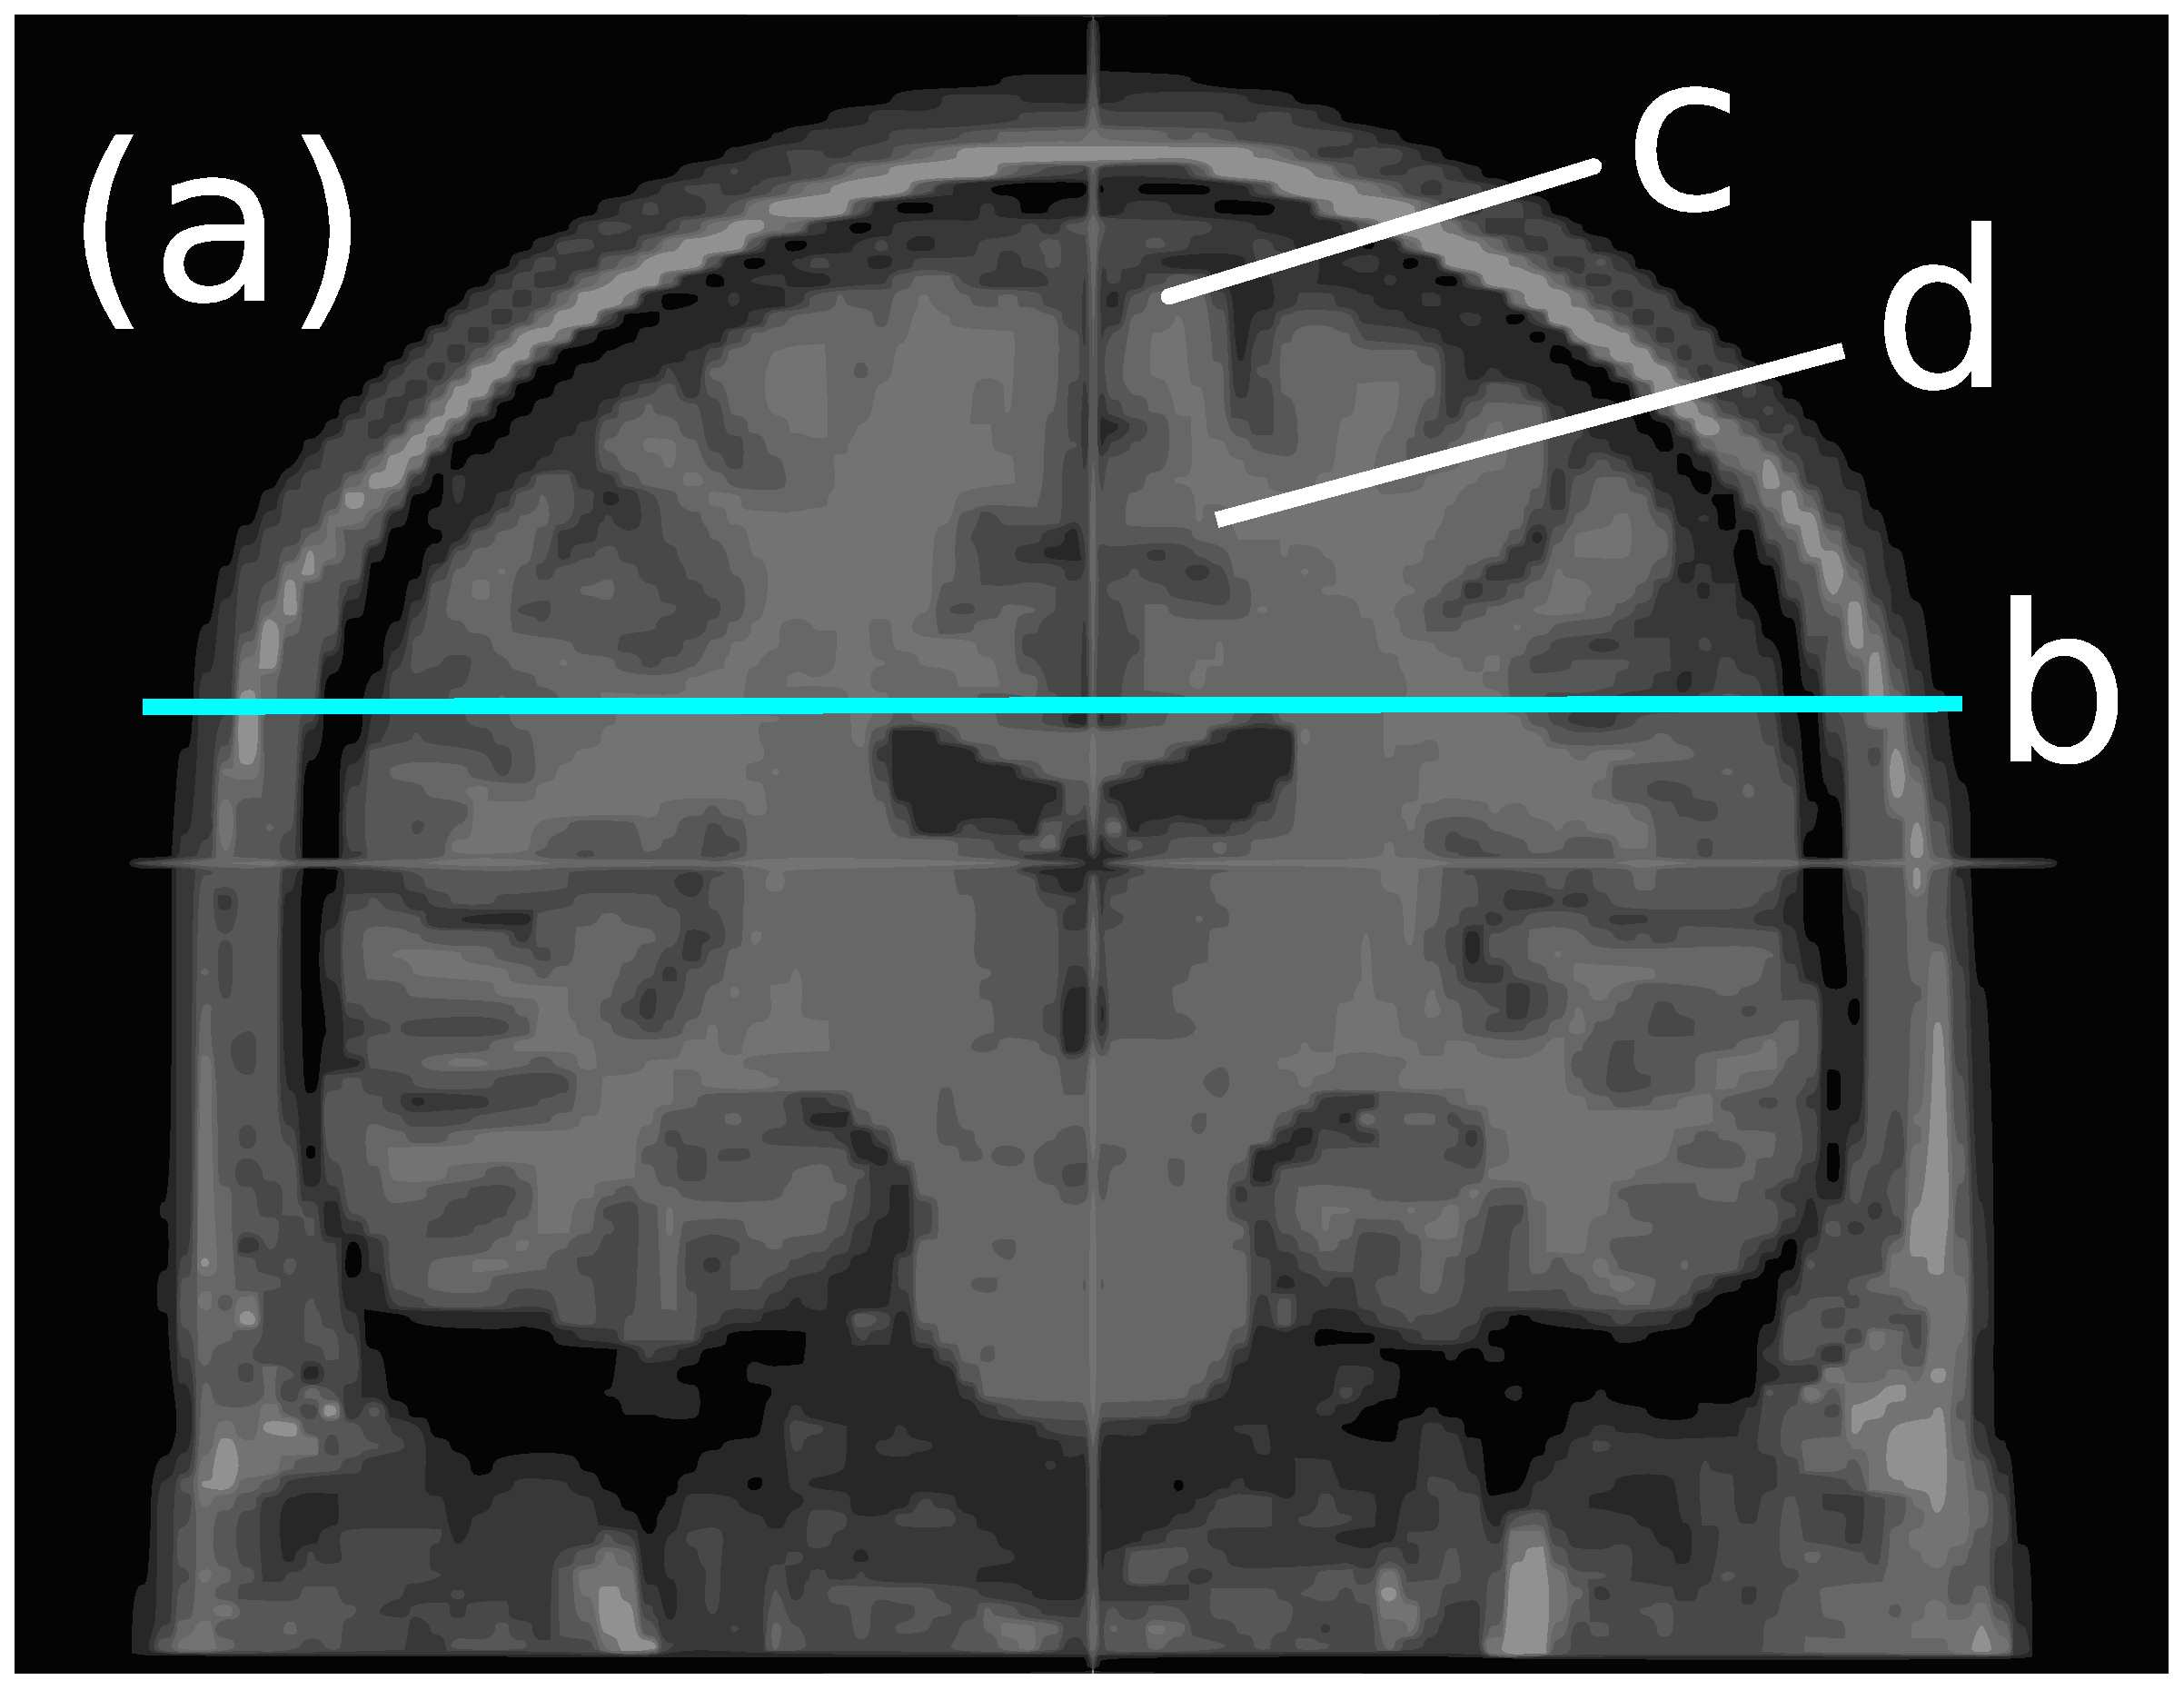
\includegraphics[width=0.36\textwidth]{headref}} & 
    			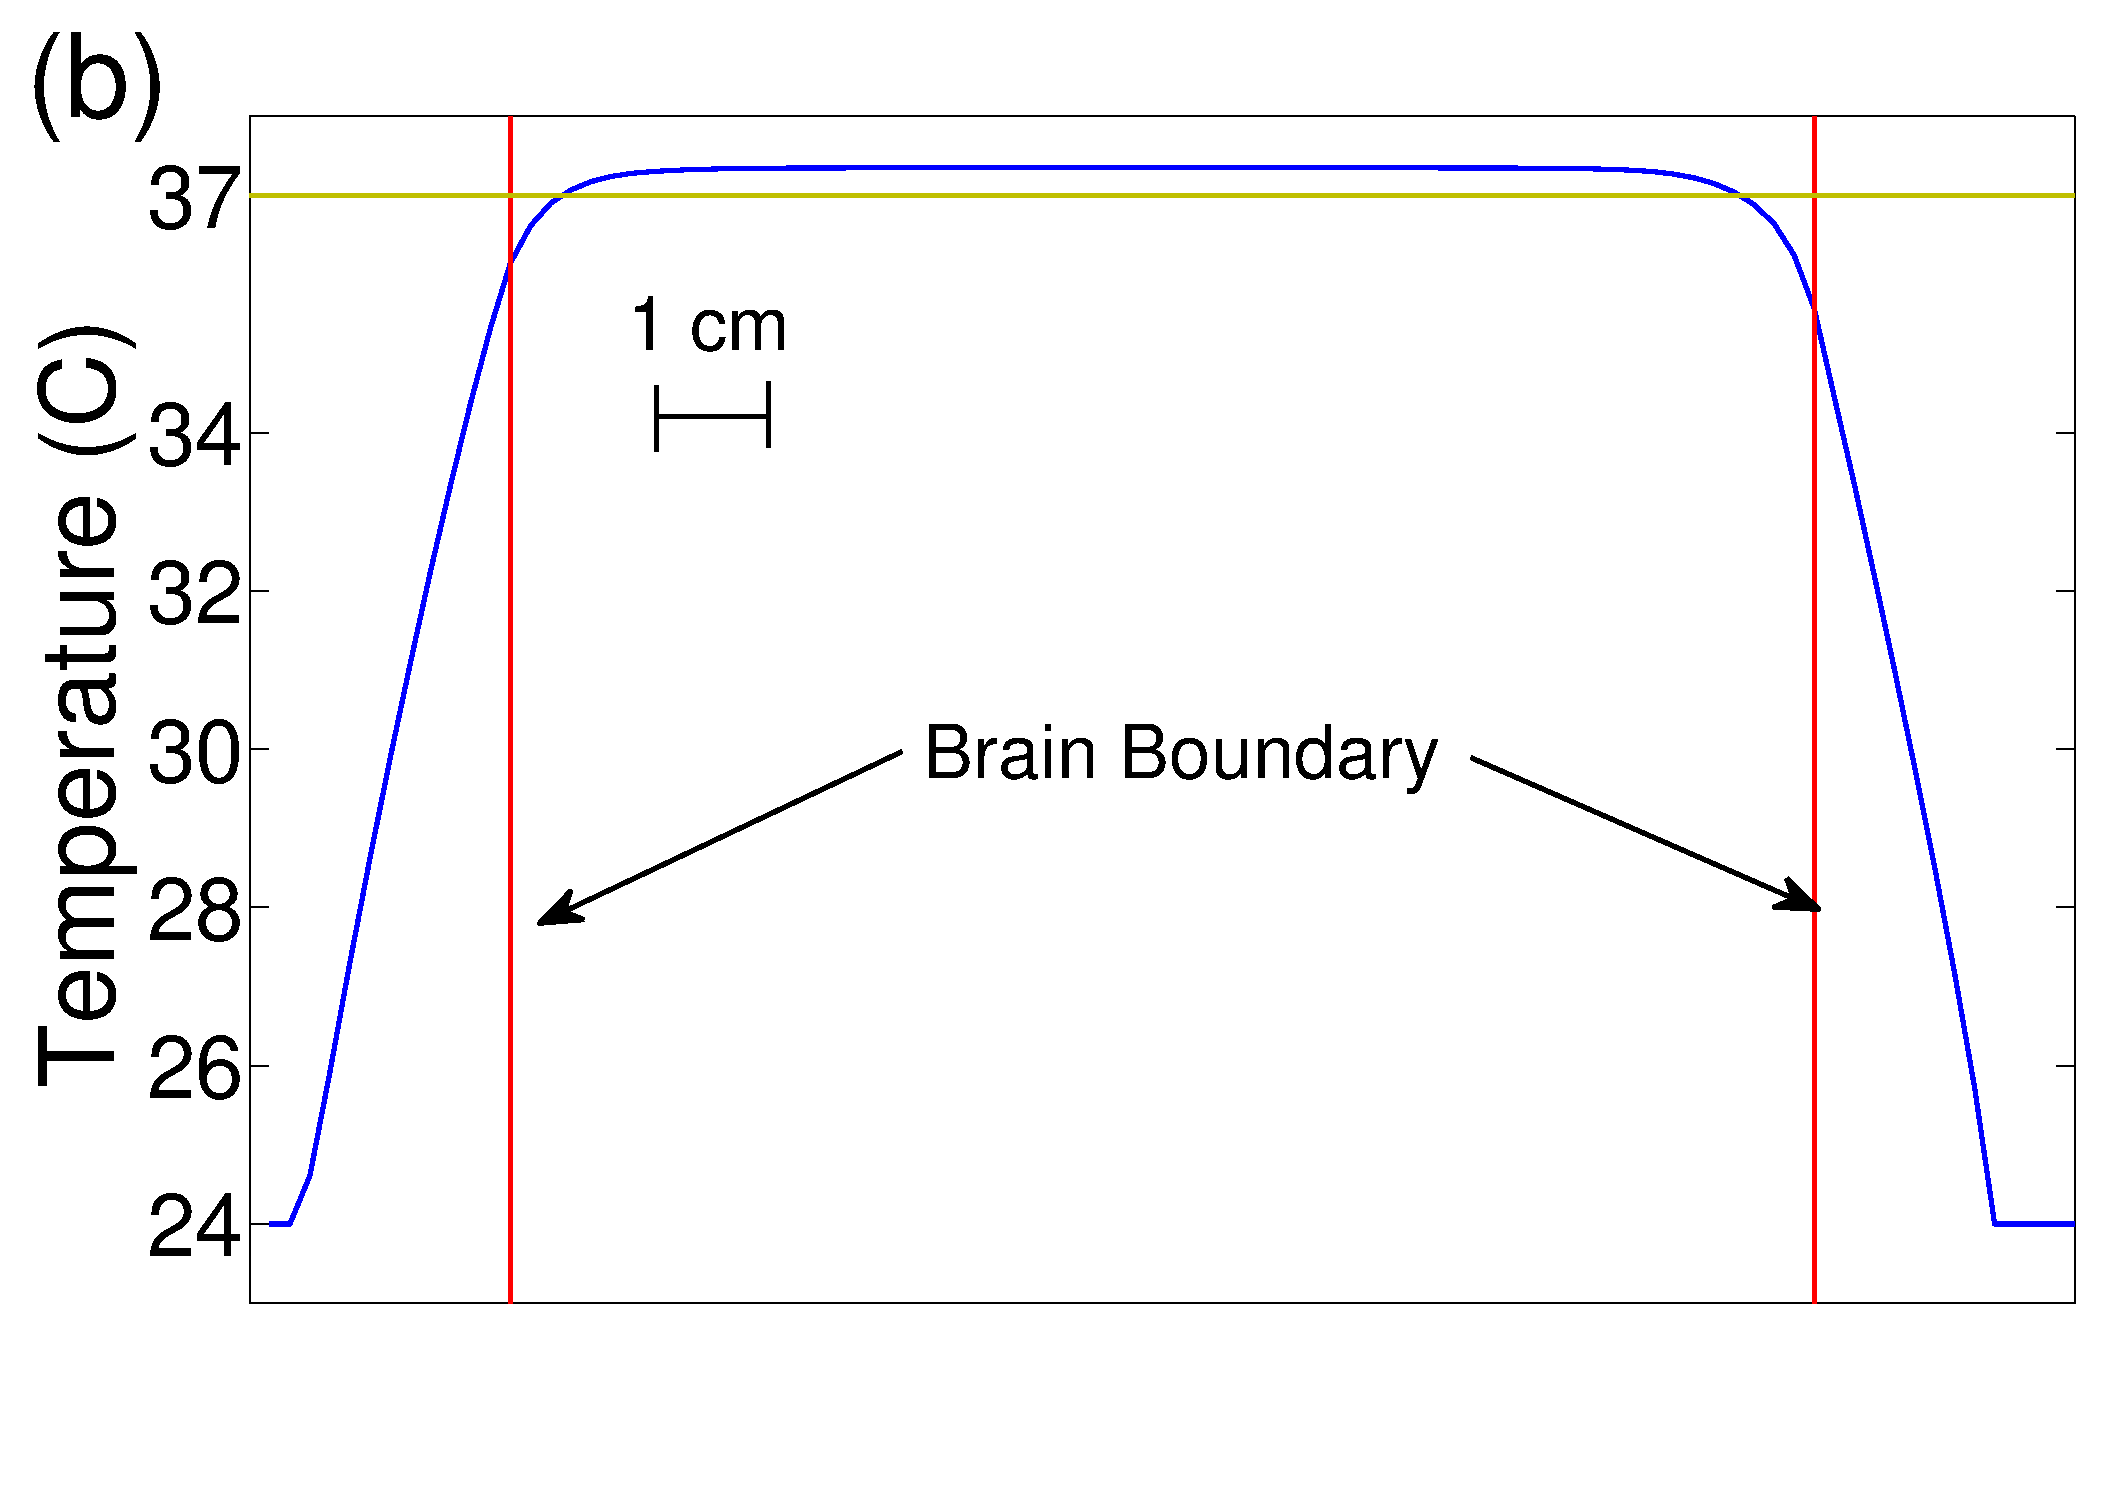
\includegraphics[width=0.5\textwidth]{equilibrium_temperature_0_55_52} \\
    			\multicolumn{2}{c}{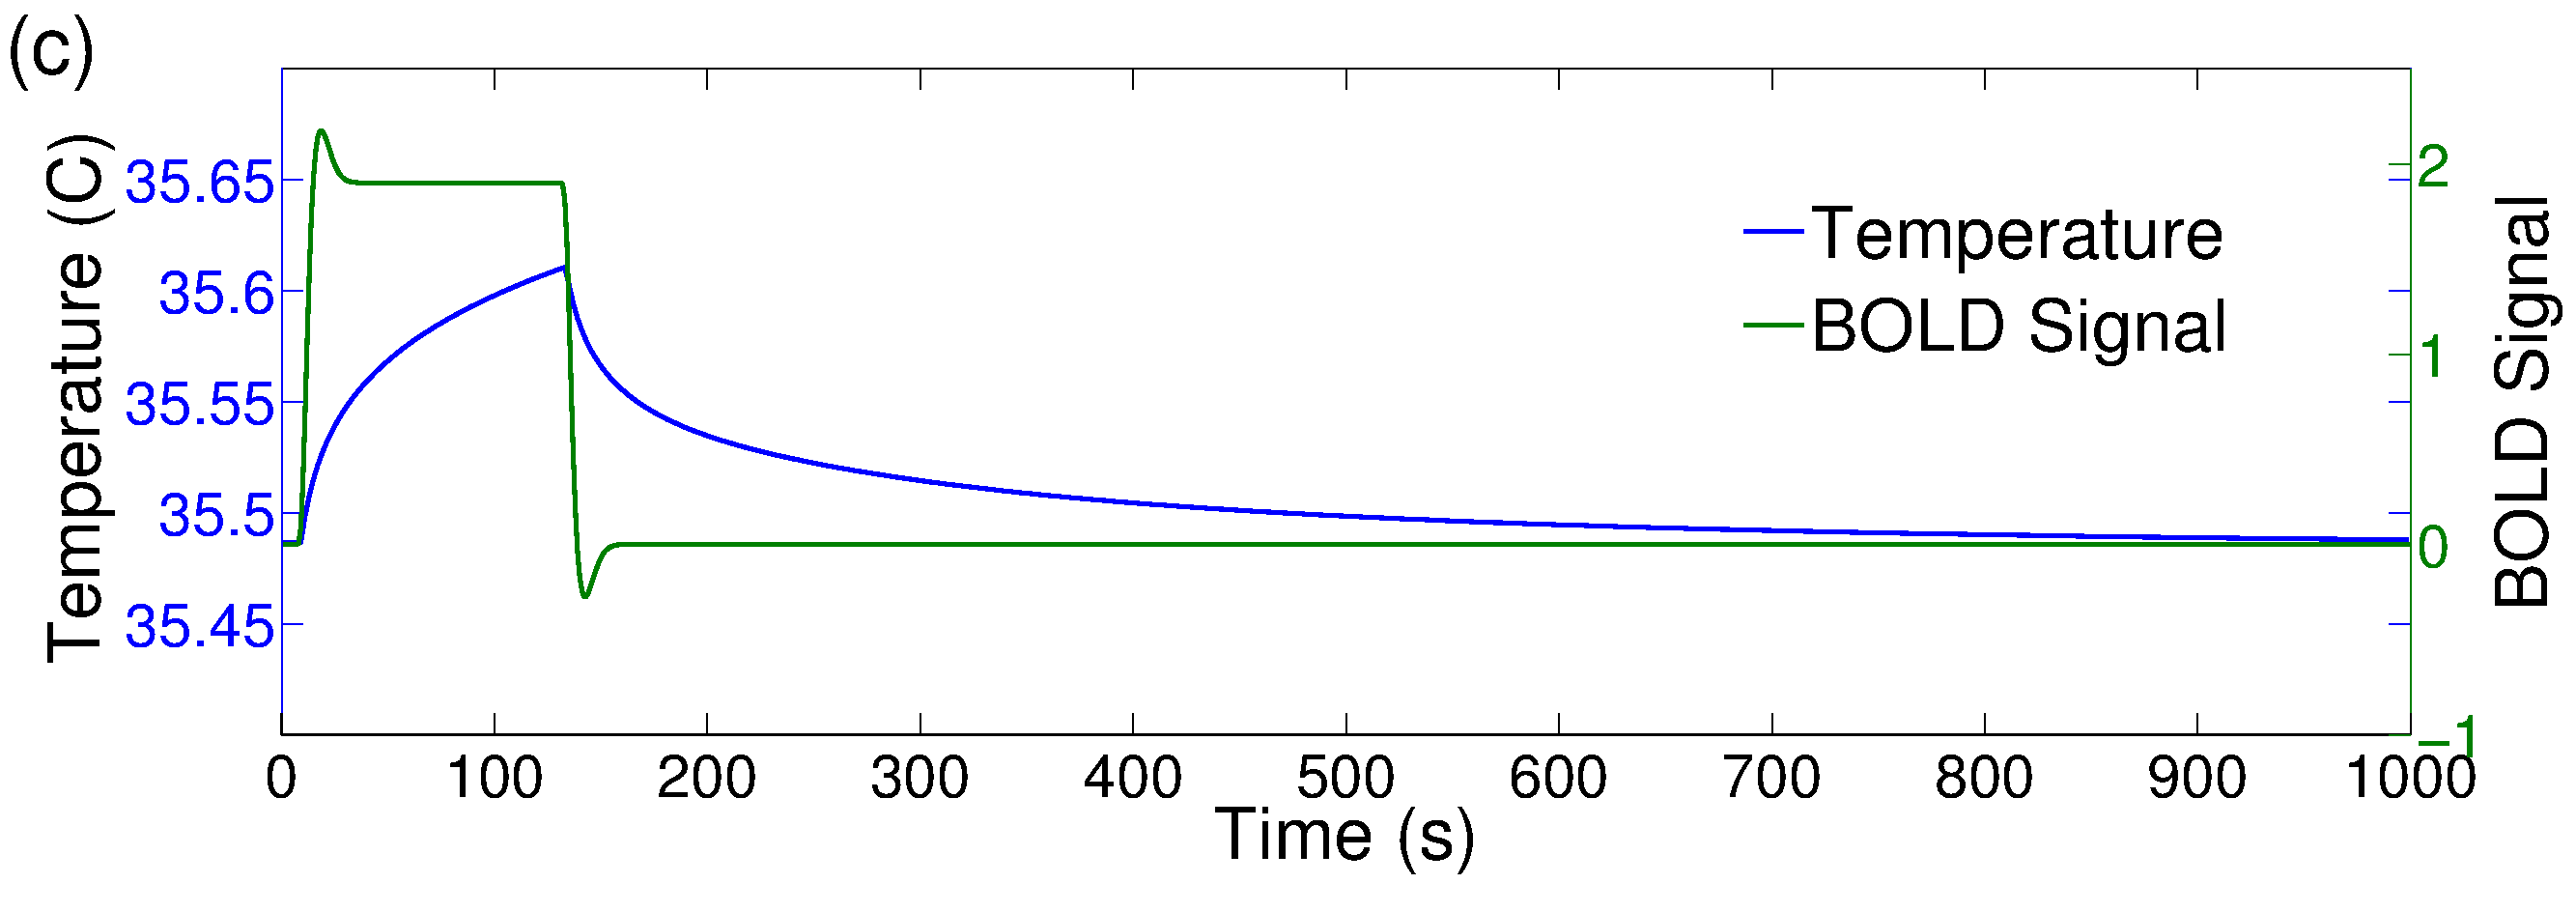
\includegraphics{sim_bold_(48_58_76)}} \\
    			\multicolumn{2}{c}{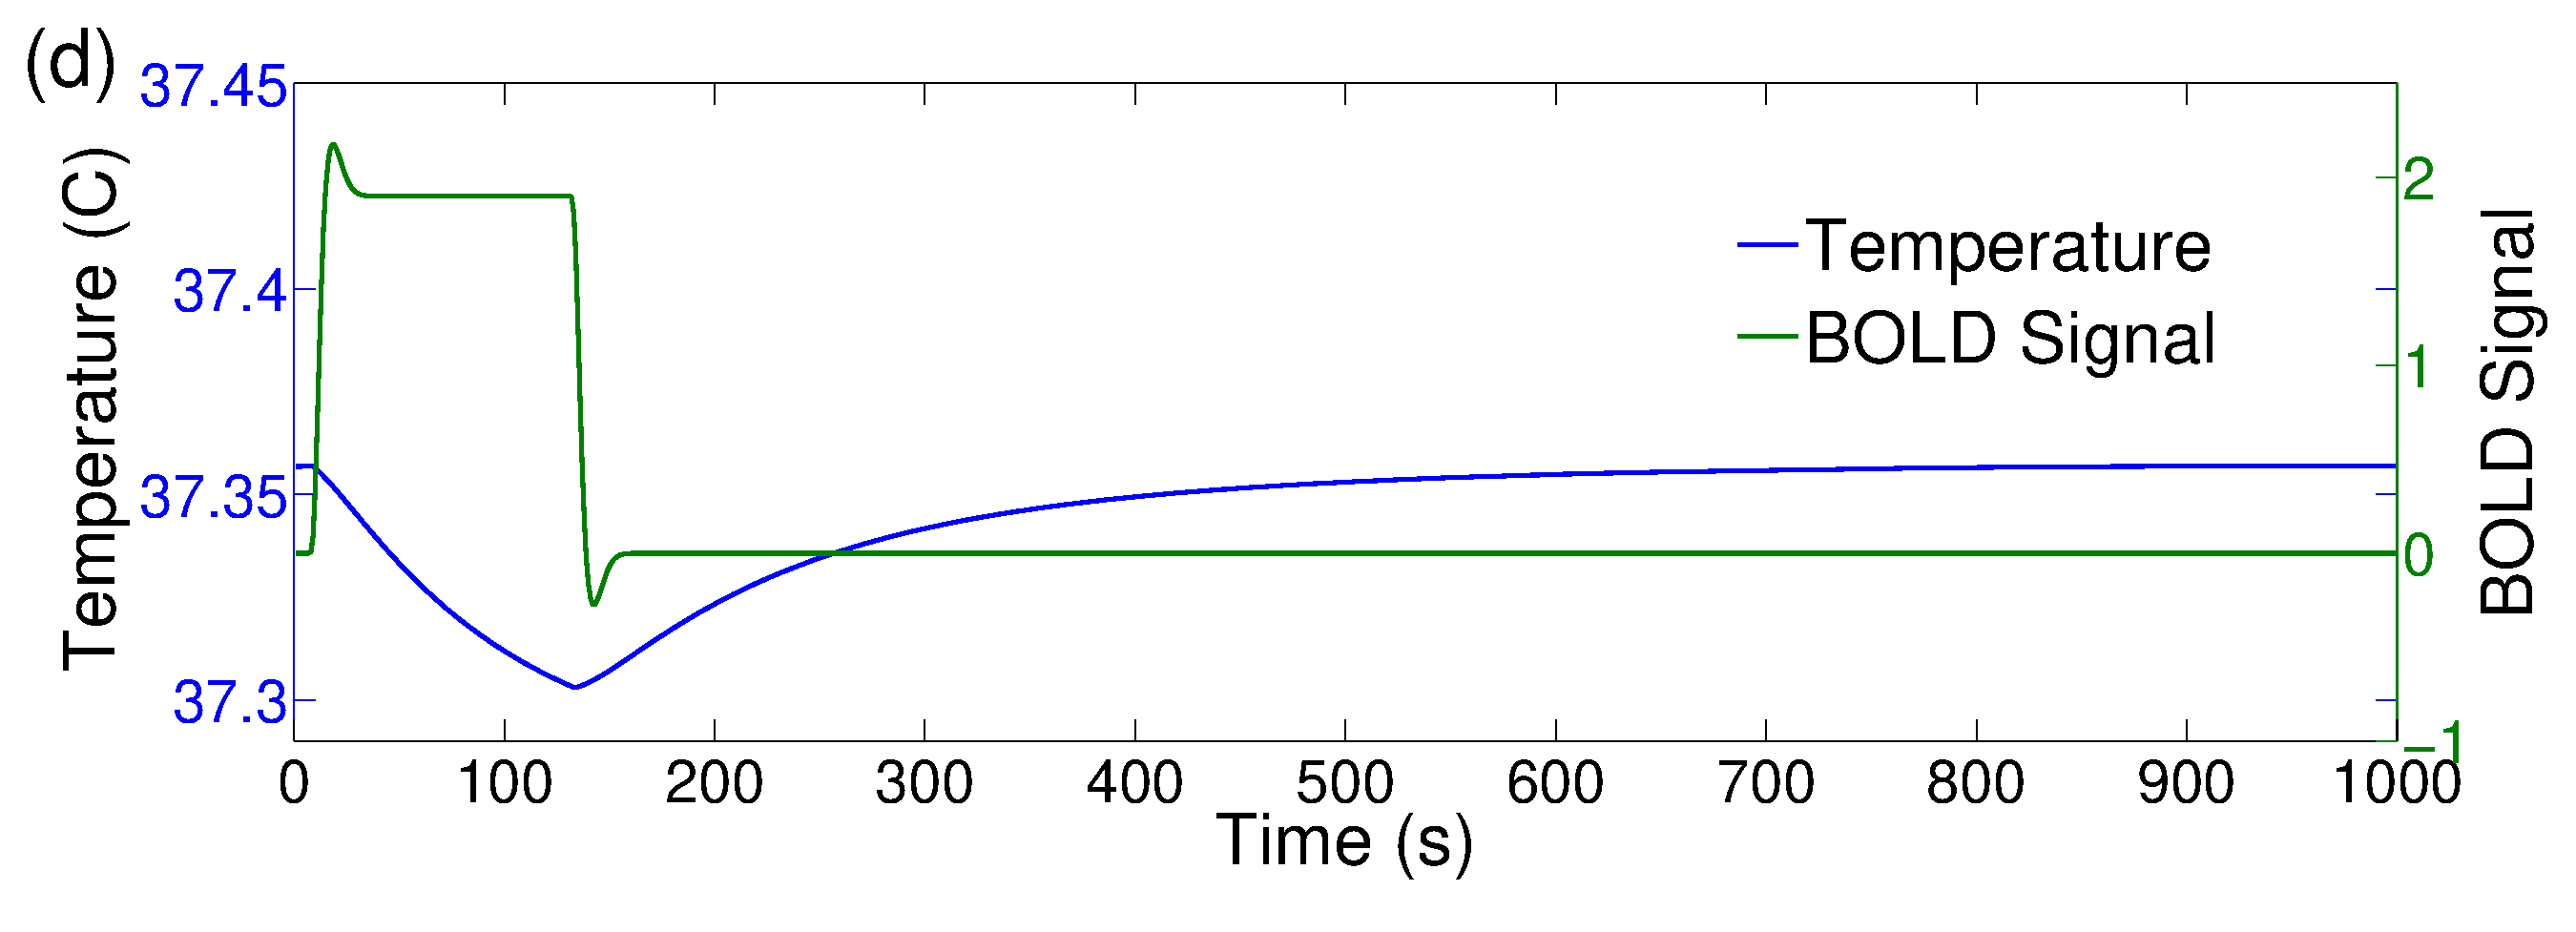
\includegraphics{sim_bold_(48_58_56)}}
    		\end{tabularx}
    	\end{center}
    	\caption[Temperature changes: simulated BOLD data]{\label{fig:simulateddata} Temperature changes using simulated BOLD signals. (a) Slice of the head (y = -12) with indicators of the locations for parts (b)-(d). (b) Equilibrium temperature along a line through the head. Red lines indicate the brain boundary and the gold line indicates the blood temperature (37\degree C) used for calculations. Inside the brain, a 4-6 mm thick shell is created where the equilibrium temperature is less than the blood temperature. Within this shell, (c) the temperature rises with increased brain activity while (d) tissue deeper in the brain experiences the opposite effect.} 
    \end{figure}
    \subsubsection{Using Experimental BOLD Data}
    \FloatBarrier
    \begin{figure}[p] 
    	\begin{center}
    		$ 
    		\begin{array}{c}
    			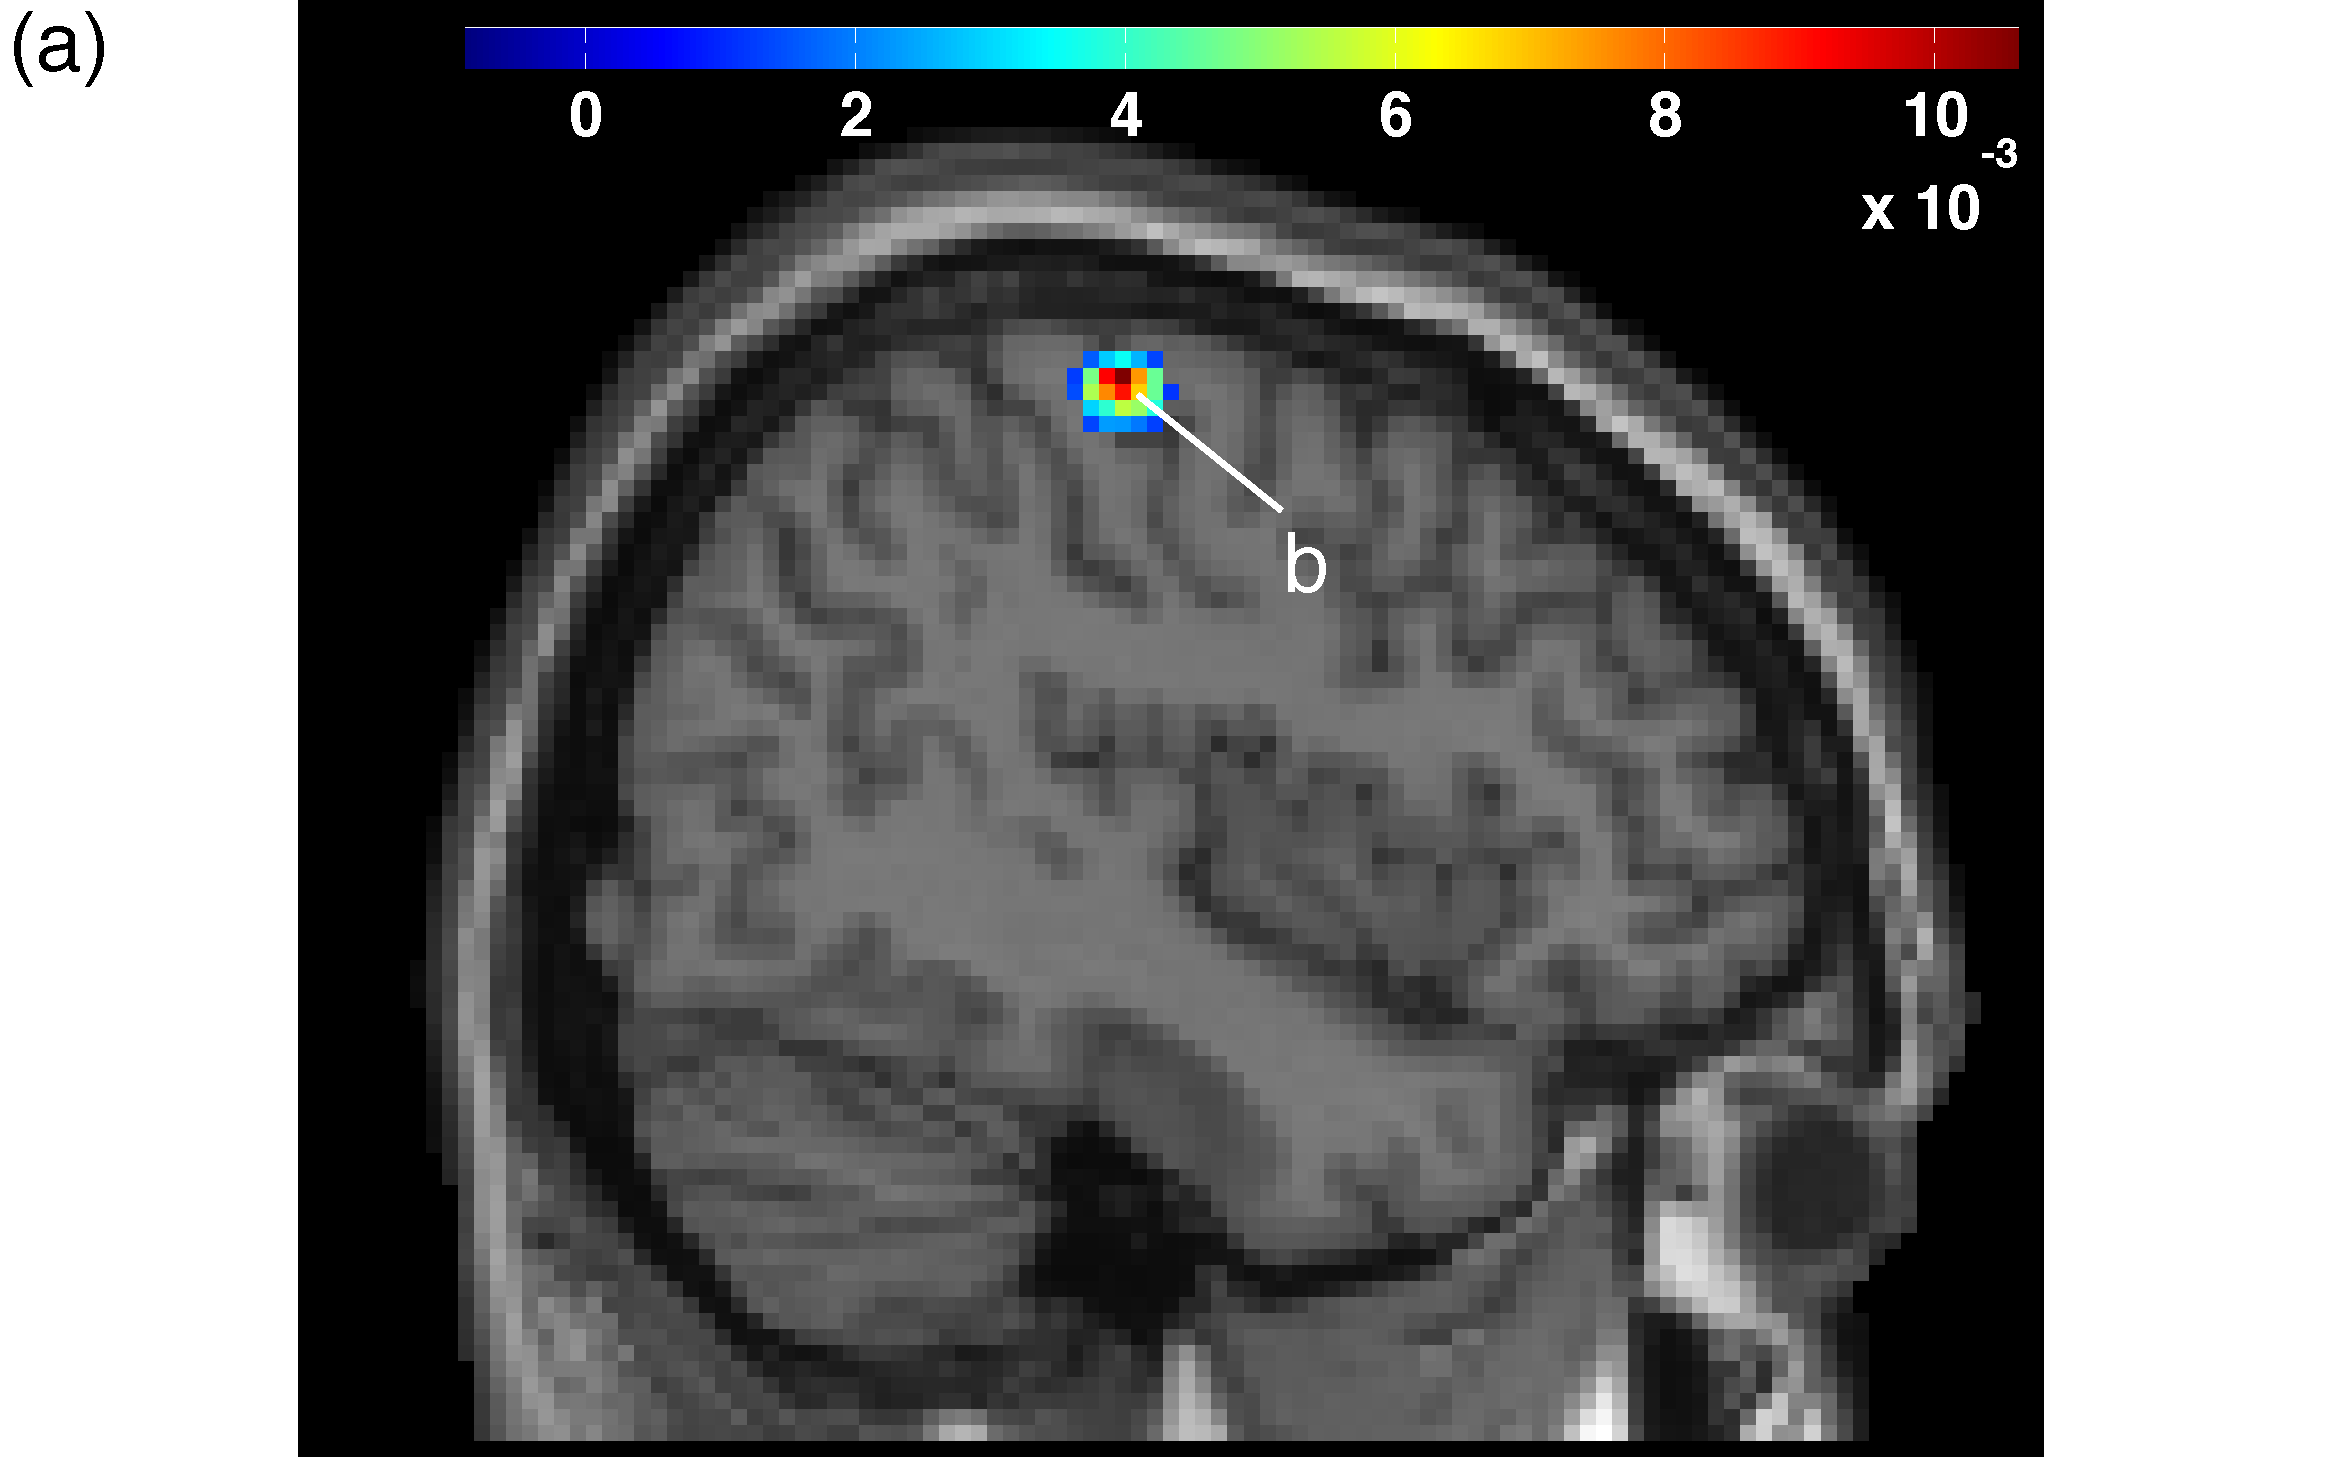
\includegraphics{slice_x_24} \\
    			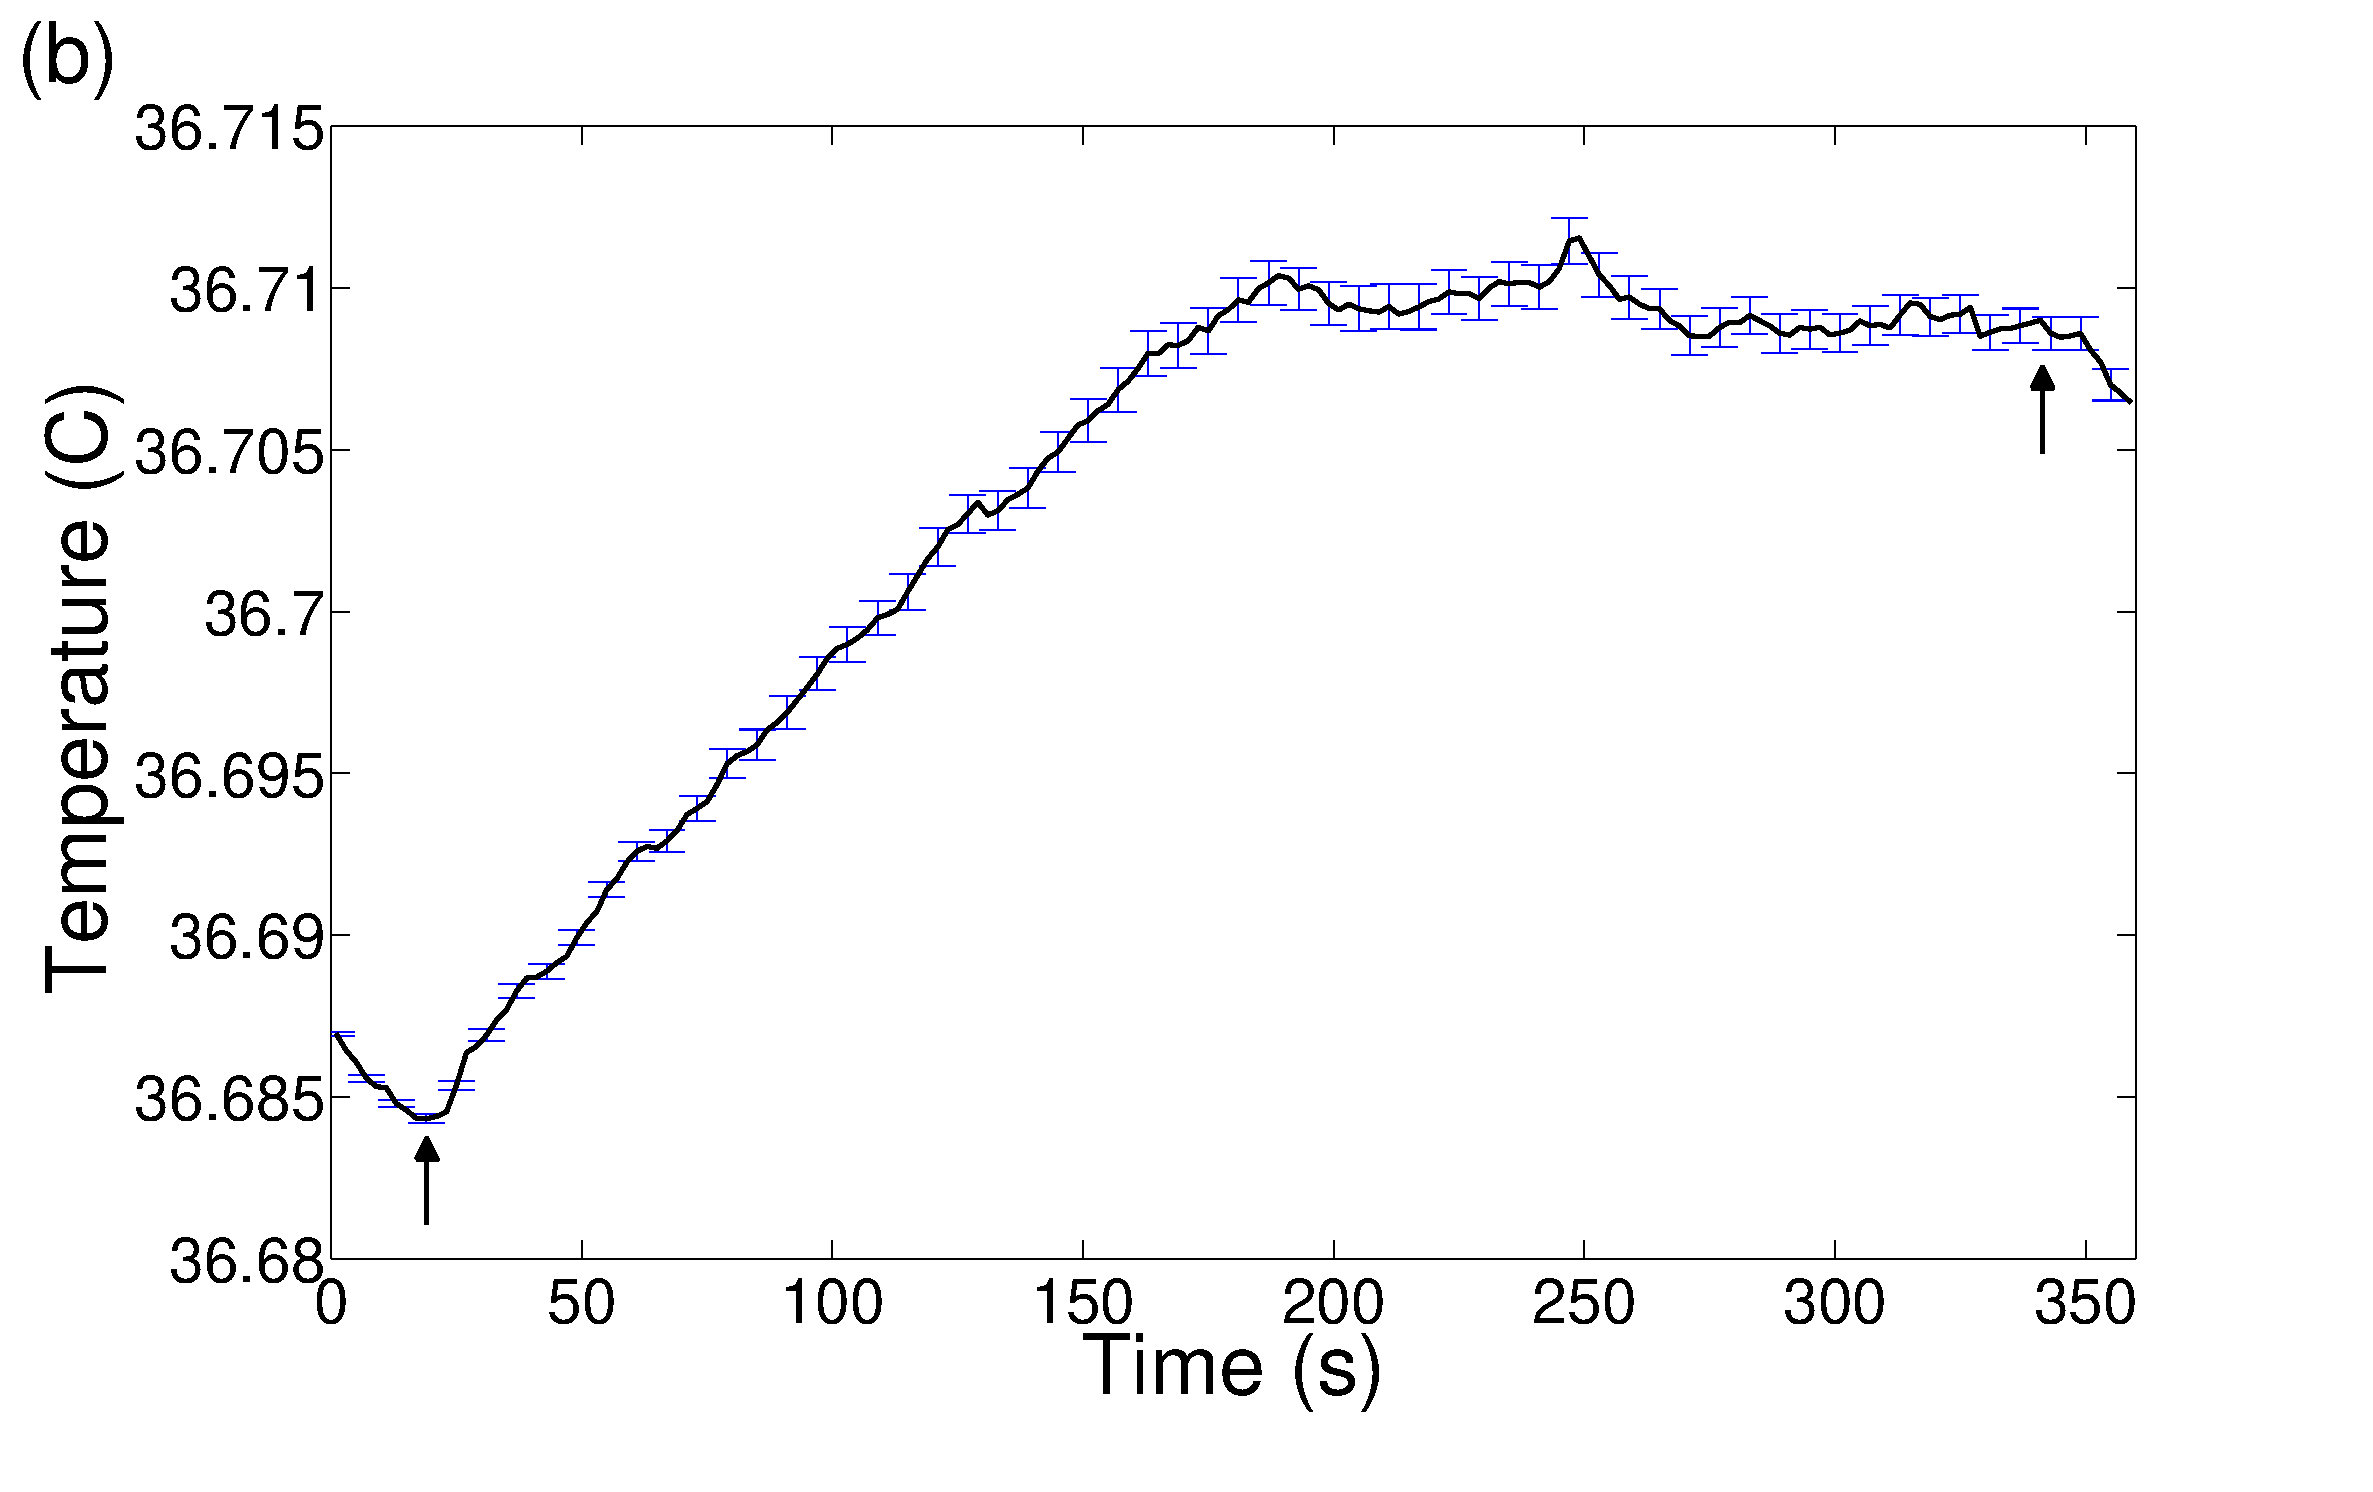
\includegraphics{avg_data_24_52_67} 
    		\end{array}
    		$ 
    	\end{center}
    	\caption[Temperature changes: experimental BOLD data]{\label{fig:realdata} Temperature calculated from a voxel within the motor cortex. (a) A slice (x = -44) showing the motor cortex warming during a finger-tapping task. (b) Temperature at a voxel within the motor cortex (-44, -24, 60) with standard error indicated by blue error bars (Arrows indicate task onset and conclusion, N=24).} 
    \end{figure}
  % talk about my approach
\chapter{Optical techniques for brain activity measurements}
\label{ch:detectors}
The best method for measuring brain temperature is to use a thermocouple probe placed in direct contact with the tissue.  Experimental measurements of brain temperature have achieved a precision of small as $0.000\,3$\degree C using this method~\citep{mcelligott}. However, this method can not be used in humans without damaging the tissue.  An optical method would be ideal for non-invasive and non-damaging measurements.  Presently, there does not exist a method for accurately measuring the temperature of brain tissues optically.  However, other optical measurements methods could be used in conjunction with a temperature model (such as the one proposed here) to calculate the temperature.  The possible application of functional Near-Infrared Spectroscopy (fNIRS) and its possible use in brain temperature calculations is discussed along with the limitations of a direct measurement technique such as thermal imaging.
  
\section{{F}unctional {N}ear-{I}nfrared {fNIR} Spectroscopy}
% detector applicaitons to improving fNIR
\begin{figure}[tb]
  \begin{center}
    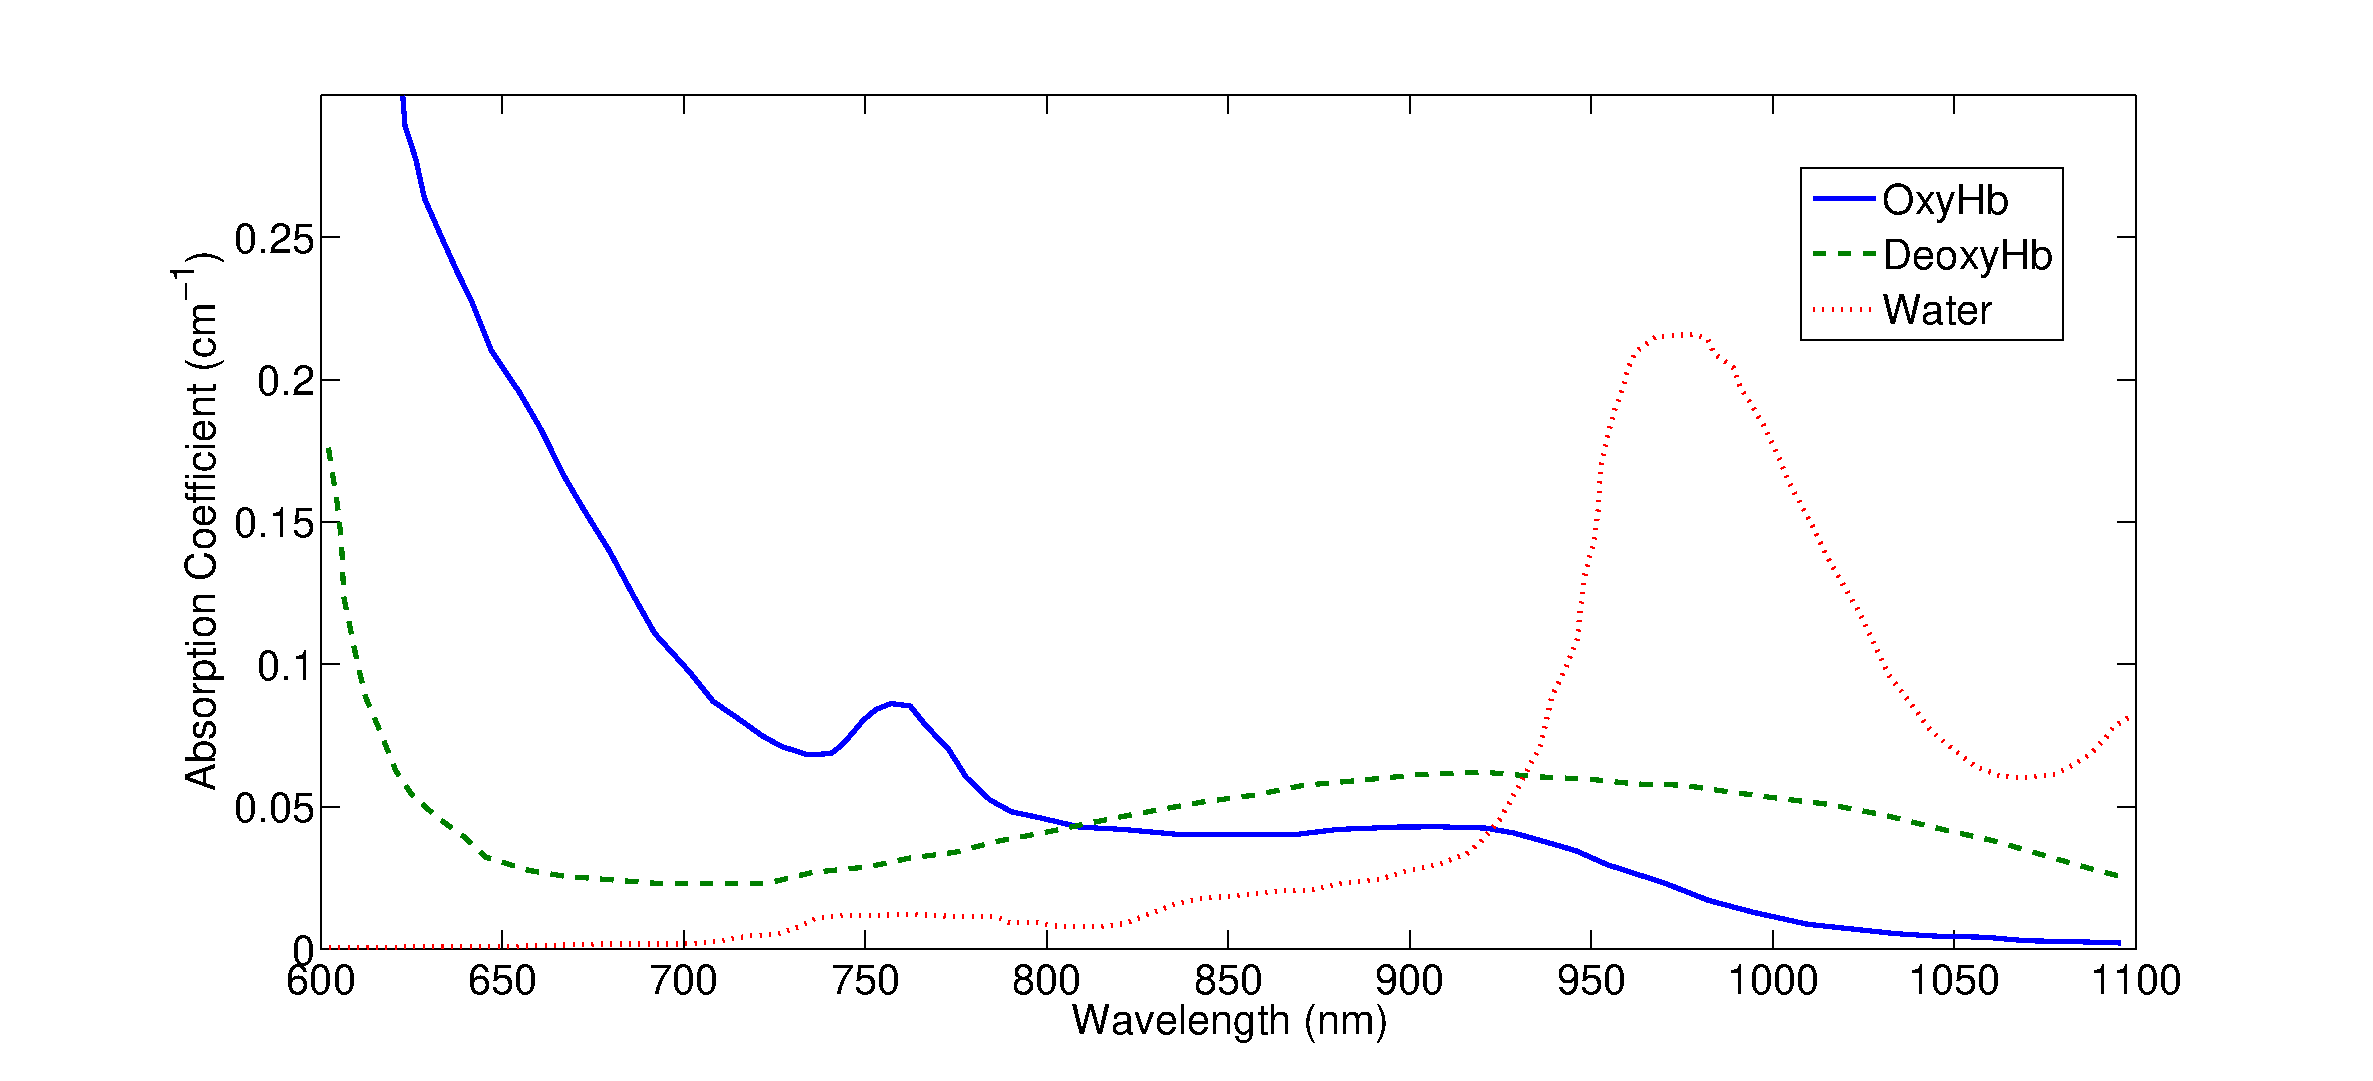
\includegraphics{AbsorptionData}
    \caption[Absorption spectra of water, deoxyhemoglobin and oxyhemoblogin]{\label{fig:fnirabsorption} Absorption spectra of water~\citet{cope}, oxyHb and deoxyHb~\citet{horecker}.}
  \end{center}
\end{figure}
\begin{table*}[tb]
  \begin{tabular*}{\linewidth}{lp{5cm}p{5cm}}
    \toprule
                         & fMRI             & fNIR            \\
    \midrule
    Spatial Resolution   & 8--27 mm$^3$  & $\sim$ 1--10 cm$^3$ \\
    Temporal Resolution  & 1--2 s        & $\sim$ 10$^{-3}$ s \\
    Measurement Parameter& blood volume, flow, and O$_2$ metabolism & oxyHb and deoxyHb concentrations \\
    Motion               & Must Remain Stationary & Small movements OK \\
    Penetration          & Whole-head    & outer 2--4 mm of brain tissue \\
    \bottomrule
  \end{tabular*}
  \caption[Comparison of fMRI and fNIR]{\label{tbl:comaparemethods}Comparison of the capabilities and limitations of fMRI and fNIR techniques.  Compiled from~\citet{bunce2006,elliott}.}
\end{table*}

As discussed in~\cref{ch:introduction}, changes in tissue activity can be detected by measuring the change in blood oxygenation levels.  Functional Magnetic Resonance Imaging (fMRI) is one technique among several for accomplishing this (the BOLD signal).

Blood oxygenation can be determined by measuring the relative concentrations of oxyhemoglobin (oxyHb) and deoxyhemoglobin (deoxyHb)~\citep{ogawa1990,kwong1992,fox1986}.  Since oxyHb and deoxyHb have different absorption spectra as shown in~\cref{fig:fnirabsorption}. These differences are possible to detect  through optical techniques.  Functional Near-Infrared Spectroscopy is a technique which utilizes two or more spectral bands in order to determine blood oxygenation.  fNIRS has a high (millisecond) temporal resolution and a low ($\sim$ 1~cm$^3$) spatial resolution compared to fMRI (as low as 1 mm$^3$). Also, fNIRS is limited to only imaging the outer cortex (2--4 mm)~\citep{bunce2006}. A comparison of fMRI and fNIR is presented in~\cref{tbl:comaparemethods}.

fNIRS works by utilizing an array of near-infrared detectors and emitters (typically spaced 2--3 cm apart) placed in contact with the skin~\citep{villringer1997,izzetoglu2004}.  A schematic of a typical fNIRS array setup is shown in~\cref{fig:fnir-arragement}. Each dashed line is a detection path and by illuminating the emitters sequentially, it is possible to have 10 detection channels using the setup shown.  The exact spacing between the emitters and detectors determines the depth the light is detected from.  As shown in~\cref{fig:fnirpenetration}, the closer the spacing, the higher the resolution but at the expense of lower penetration.  Conversely, in order to detect light passing through deeper tissue, a wider spacing is used which reduces the resolution.  The exact wavelengths used vary, but all lie within an optical window between 700--1000~nm~\citep{villringer1997} where the near-infrared photon absorption in the tissue is low~(\cref{fig:fnirabsorption}).

\begin{figure}[tb]
  \centering
  \tikzstyle{detector} = [circle,draw, ultra thick, fill=blue!20]
\tikzstyle{ann} = [draw=none,fill=none,right]
\tikzstyle{led} = [star,star points=10,draw, thick, fill=red]
\tikzstyle{l} = [draw, very thick, color=black, dashed]
\tikzstyle{legend-box} = [rectangle, draw, thick, fill=none, minimum height=2cm, minimum width=3.5cm]
\begin{tikzpicture}
  \matrix[row sep=1.5cm,column sep=1.5cm] {
  \node[detector] (d11) {}; & &
  \node[detector] (d12) {}; & &
  \node[detector] (d13) {}; & &
  \node[detector] (d14) {}; \\
  & \node[led] (e1) {}; &
  & \node[led] (e2) {}; &
  & \node[led] (e3) {}; \\
  \node[detector] (d21) {}; & &
  \node[detector] (d22) {}; & &
  \node[detector] (d23) {}; & &
  \node[detector] (d24) {};\\
  };
  \node[ann, right=of d11, yshift=-1cm] {$l$};
  \node[detector, right=of d14, yshift=-1.2cm] (dRef) {};
  \node[led, below=of dRef, yshift=0.7cm]      (eRef) {};
  \node[ann, right=of dRef, xshift=-0.9cm] {Detector};
  \node[ann, right=of eRef, xshift=-0.9cm] {Emitter};
  \node[legend-box, right=of d14, yshift=-1.6cm, xshift=-0.5cm]{};
  \path[l](d11.south east) -- (e1.north west);
  \path[l](d12.south west) -- (e1.north east);
  \path[l](d12.south east) -- (e2.north west);
  \path[l](d13.south west) -- (e2.north east);
  \path[l](d13.south east) -- (e3.north west);
  \path[l](d14.south west) -- (e3.north east);
  \path[l](d21.north east) -- (e1.south west);
  \path[l](d22.north west) -- (e1.south east);
  \path[l](d22.north east) -- (e2.south west);
  \path[l](d23.north west) -- (e2.south east);
  \path[l](d23.north east) -- (e3.south west);
  \path[l](d24.north west) -- (e3.south east);
\end{tikzpicture}
  \caption[Arrangement of detectors and emitters in a typical fNIRS setup]{\label{fig:fnir-arragement}Arrangement of detectors and emitters in a typical fNIRS setup. Light coming from emitters (stars) is detected by the detectors (circles) set at a distance $l$ away.}
\end{figure}
\begin{figure}[tb]
  \centering
  \includegraphics{fnir-penetration}
  \caption[Penetration by fNIR]{\label{fig:fnirpenetration}Penetration depth of a fNIR detector as a function of the distance between the NIR emitter and detector.  Light emitted from the left passes through the tissue before it is detected.  The path it takes through the tissue is determined by the distance between the emitter and detector.  A larger separation (L$_2$) allows the light to penetrate deeper tissues (d$_2$).  Modified after~\citep{head2010}}
\end{figure}

Three techniques are used to illuminate the tissue: (i)~time domain (or time resolved spectroscopy, TRS), (ii)~frequency domain and, (iii)~continuous wave illumination~\citep{izzetoglu2004}.  In TRS, short pulses of light are incident on the tissue and the temporal distribution of photons in measured.  In frequency domain spectroscopy, the amplitude of the indecent light is modulated at a high frequency (10--100~MHz) and the phase shift and amplitude decay of the detected light is compared to the incident light~\citep{boas2002}. In continuous wave illumination, the incident light is not modulated so the detected light can only be compared for amplitude attenuation~\citep{izzetoglu2004}.

All of the techniques use the Beer-Lambert Law~\citep{beerlambert}
\begin{equation}
  I = I_0 e^{-\alpha (\lambda) x} \label{eq:beerlambert1}
\end{equation} 
modified to isolate the contributions from oxyHb and deoxyHb~\citep{cope}:
\begin{equation}
  \label{eq:modifiedbeerlamber}
  I = G I_0 e^{-(\alpha_{deoxyHb}C_{deoxyHb}+\alpha_{oxyHb}C_{oxyHb})L} 
\end{equation}
where G is a factor to adjust for the measurement geometry, $I_0$ is in the incident light intensity, $\alpha_{oxyHb}$ and $\alpha_{deoxyHb}$ are the molar extinction coefficients for oxyHb and deoxyHb, $C_{oxyHb}$ and $C_{deoxyHb}$ are the chromophore concentrations for oxy-Hb and deoxy-Hb, and L is the path length~\citep{izzetoglu2004}.  By comparing a baseline measurement~($I_b$) with a new measurement~($I$), the optical density can be determined~\citep{izzetoglu2004}
\begin{equation}
  \Delta OD = \log \frac{I_b}{I} = \alpha_{deoxyHb} \Delta C_{deoxyHb}+\alpha_{oxyHb} \Delta C_{oxyHb}
\end{equation}
As discussed in~\citet{izzetoglu2004}, at least two wavelengths are utilized in the spectral window (700--1000~nm) in order to determine the change in concentration of chromophores $\Delta C_{deoxyHb}$ and $\Delta C_{oxyHb}$.  With these values, the oxygenation and total blood volume can be determined:
\begin{align}
  \label{eq:o2bloodvolume}
  Oxygenation\ &= \Delta C_{HBO2} - \Delta C_{HB} \nonumber \\
  Blood\ Volume\ &= \Delta C_{HBO2} + \Delta C_{HB} 
\end{align}
Using this method to experimentally measure the blood oxygenation while measuring the fMRI BOLD response could be used to refine the present model for calculating the metabolism and blood flow from the BOLD response.

While fNIRS does not provide spatially-precise measurements as fMRI, it should be possible to modify the existing model for calculating temperature from the BOLD response to use fNIR data. This would be advantageous because fNIRS systems are cheaper and less disruptive than fMRI systems, meaning they can be used with a wider range of patients (children and the elderly).  For this reason, developing a model which uses fNIRS data should be considered in future research.

\section{Thermal Imaging}

The primary challenge in brain temperature research is preforming brain temperature experimental measurements.  Since it is non-invasive, thermal imaging is appealing as a possible replacement for damaging thermocouple probes.  Unfortunately, this technique is limited by the high absorption of mid-infrared photons by water.

Light absorption by a material is modeled using the Beer-Lambert law
\begin{equation}
  I = I_0 e^{-\alpha (\lambda) x} \label{eq:beerlambert}
\end{equation}
where $I$ is the intensity at a depth $x$ remaining from light with an incident intensity $I_0$ in a material with absorption coefficient $\alpha$.  The point at which the intensity has decayed to 1/$e$ (about 37\%) of the incident intensity is called the penetration depth, $\delta_{p}$
\begin{equation}
  \delta_p = \frac{1}{\alpha (\lambda)} \label{eq:penetrationdepth}
\end{equation}
This equation can be used along with the black-body spectrum at tissue temperatures (\cref{fig:blackbody}) we can estimate the penetration depth of mid-infrared photons passing through water.

\begin{figure}[tb]
  \centering
  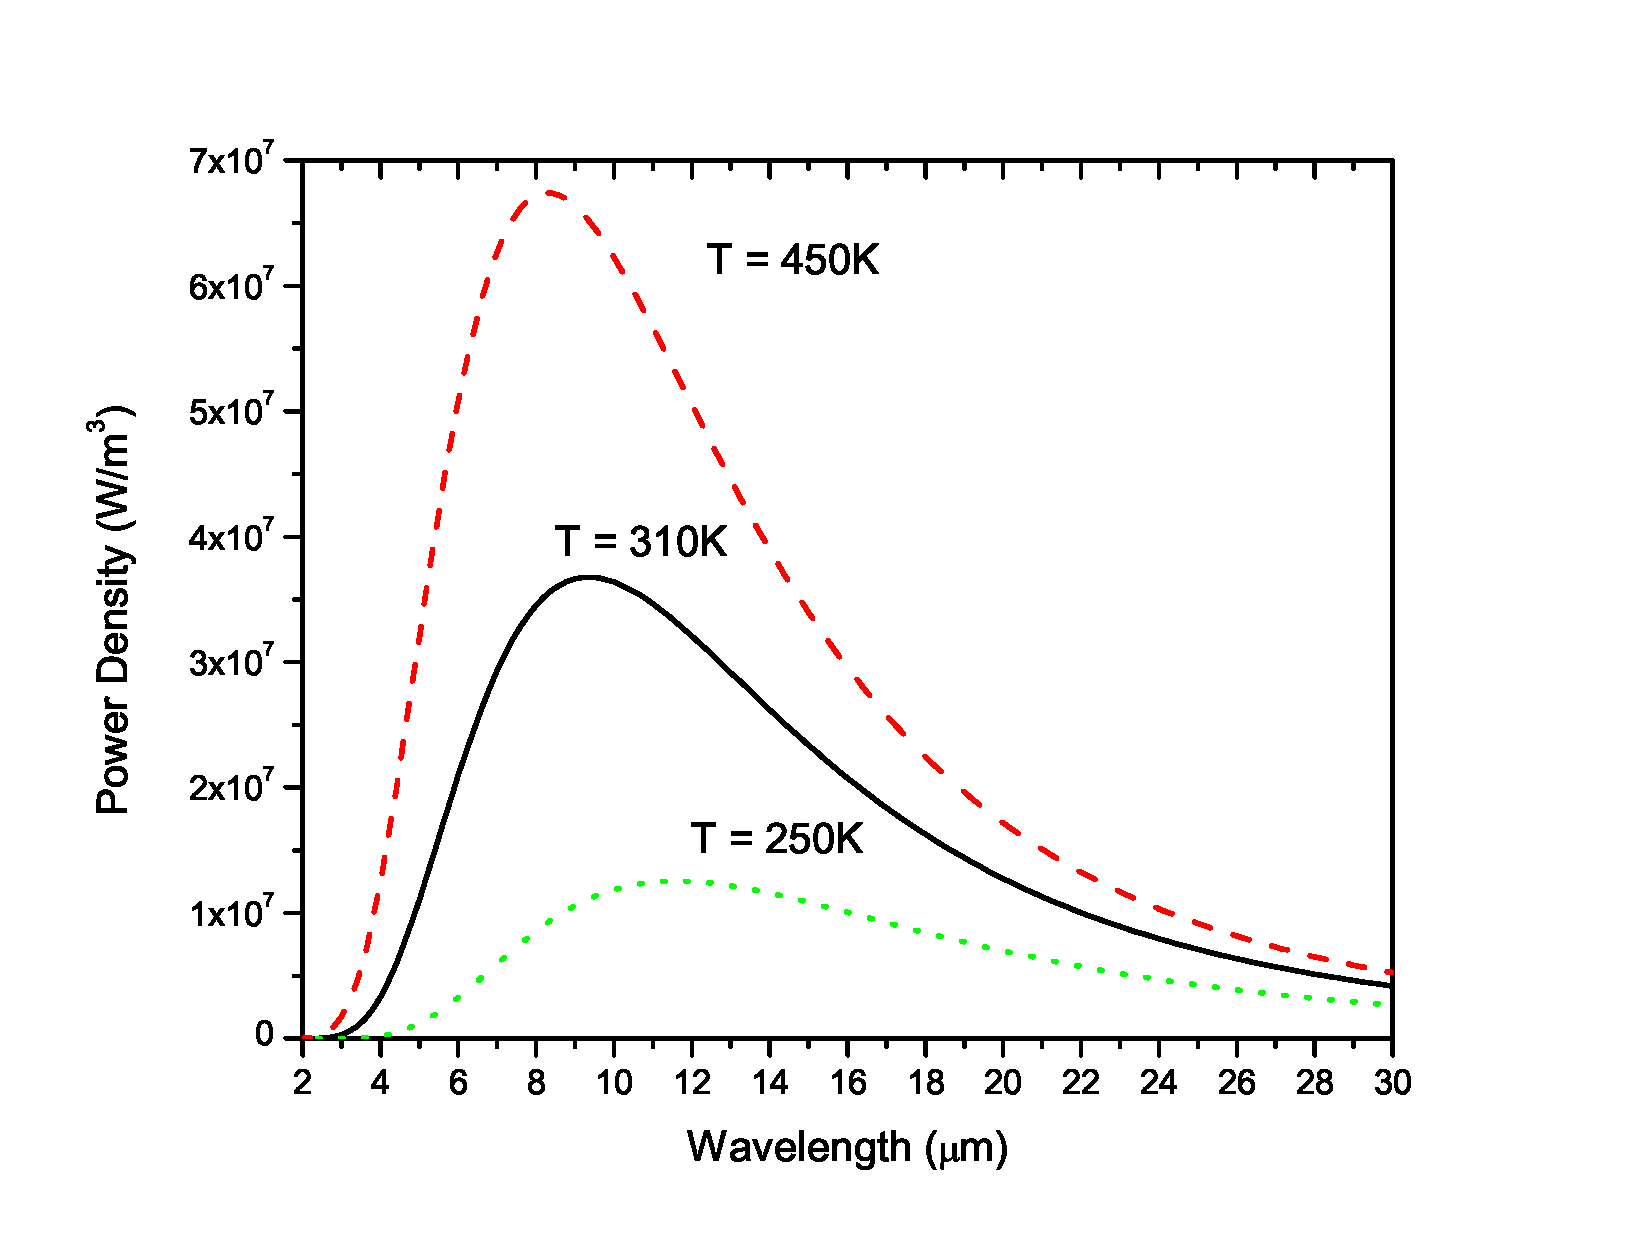
\includegraphics{blackbody}
  \caption[Black-body Spectrum at 250, 310 and 350 K]{\label{fig:blackbody}Black-body spectrum at 250, 310 and 350 K calculated using Planck's Law.}
\end{figure}
\begin{figure}[tb]
  \centering
  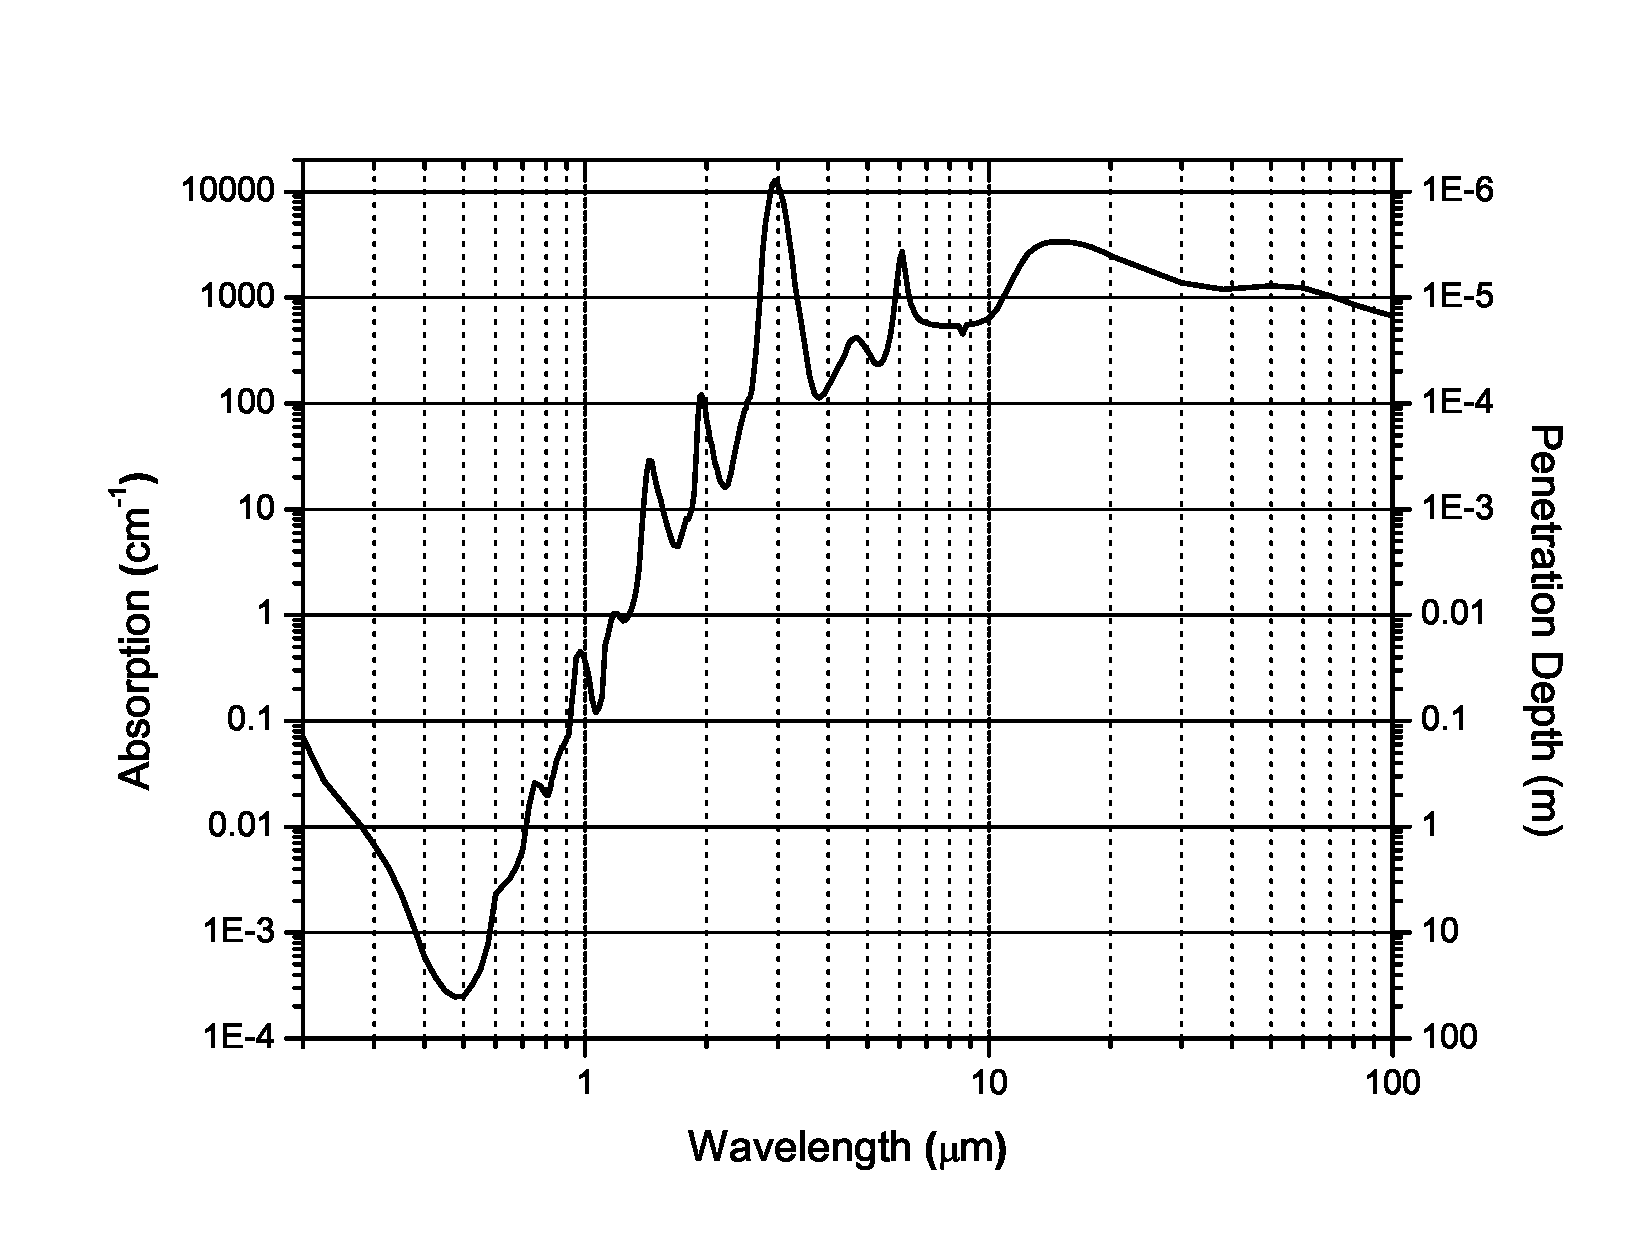
\includegraphics{water-wide-band}
  \caption[Wide-band absorption spectra of water]{\label{fig:waterabs}The absorptions spectra of water from UV to far-infrared.  Modified from~\citet{hale73}.}
\end{figure}

Wien's Displacement Law is a solution to Planck's law for the peak light emission wavelength:
\begin{align}
  \lambda_{max} &= \frac{b}{T} \label{eq:wienslaw} \\
  b &= 2.897\,7721 * 10^{-3} \mbox{ K m} \nonumber
\end{align}
where $b$ is Wien's displacement constant and T is the temperature in kelvin.  For $T=310$~K ($T=37\degree$~C), Wien's law yields a peak black-body emission wavelength of 9.347$\,$652~\textmu m. A physiologically reasonable temperature change to expect from stimulation is on the order of 0.01\degree C which would correspond to a new peak wavelength of 9.347$\,$350~\textmu m (T=310.01 K) or a shift of 0.302 nm.

The values of the absorption coefficient and the penetration depth of photons in water is shown in~\cref{fig:waterabs}. Looking at around 9.3~\textmu m, the absorption coefficient is approximately 700 cm$^{-1}$ which corresponds to a penetration depth of approximately 0.14~\textmu m.  This depth is roughly five orders of magnitude smaller than the distance from the surface of the brain to the surface of the head.  Further, all photons emitted as blackbody radiation (ranging from 3~\textmu m to over 30~\textmu m) have a penetration depth of less than 100 microns.  Thus, a thermal imaging camera is unable to image photons coming from the brain.

When thermal imaging is used, the photons collected come from the skin of the head rather than from any deeper tissues, thus it is not a viable form of brain activity detection unless direct line of sight to the brain is available (such as in an open skull surgery).  The noise-equivalent temperature difference (NETD) of currently available cameras is greater than 14~mK~\citep{flir,ici} so it would be limited to only the most extreme of excitations even if line of site to the brain is available.  As a comparison, the finger-tapping task discussed in the results section (\cref{sec:experimentalresults}) only induced a peak temperature change of 25~mK after tapping for about 170~seconds.  Detection of this activity would be at the limits of a thermal imaging camera.

While its applications to detecting brain activity are limited, thermal cameras could be useful in the operating room.  It has been found that inducing mild hypothermia in patients being treated for cerebral ischemia improves the clinical outcome~\citep{maher1993}. The same treatment has been shown to improve the outcome of patients who have experienced a stroke~\citep{krieger2001} and even in patients with severe head injuries~\citep{soukup2002}. The temperature of the brain is currently inferred from the core body temperature (which is monitored via an invasive thermistor catheter). If it is possible to directly image the brain (i.e. during surgery) then the hypothermia treatment can be better monitored through a thermal imaging camera.  This would be especially useful since conductive and radiative heat loss to the air from an exposed brain could reduce how tightly the brain temperature is regulated by the arterial blood temperature.

Optical detectors face many challenges working with biological tissue, the worst being infrared light absorption by water. fNIRS works within an optical window in the water absorption in order to measure changes in blood oxygenation, while thermal imaging is limited to measuring the temperature of tissue it has direct line of sight with because of the high absorption of water in the operating window. Despite their limitations, both of these techniques could be used in future studies to improve our understanding of brain temperature dynamics.
\chapter{Conclusion}

It has been shown that by considering the entire head within the model, brain temperature can be reliably calculated from non-invasive fMRI measurements. Experimental measurements of activity-induced brain temperature changes have shown that a simple relationship does not exist~\citep{mcelligott,kiyatkin,zeschke,george,tachibana}. Single-voxel brain temperature modeling efforts predict that an increase in brain activity will induce a decrease in temperature. This one-dimensional perspective does not account for the spatial distribution of heat throughout the head like a multi-voxel approach.

Our model of brain temperature changes is able to account for the variability found in experimental brain temperature measurements.  This is accomplished by modeling heat dynamics throughout the entire head rather than reducing the model to one ROI.  It was found that the variability in experiment measurements is most likely due to differences in resting state temperatures throughout the brain.  Since each voxel is at a slightly different temperature, the same change in the BOLD response may result in different changes in temperature. Additionally, it was found through the model that a thin (4--6 mm) region of outer cortical tissue is at a resting temperature below the blood temperature.  In this region, an increase in brain activity (inducing an increase in CBF) will warm the tissue.  Thus, with the same BOLD response, tissue may either be warmed or cooled depending on it's proximity to the surface of the head.

The biggest shortcoming of our model is that we are unable to independently compare our calculations with experimental measurements of temperature and BOLD response. It was not possible for us to do this because there is currently not a method for non-invasively measuring temperature independent of an fMRI. An improvement to the model could also be gained by a more accurate method of CMRO$_2$ and CBF calculations from the BOLD response. The current method uses empirically fit formulas, so the accuracy is limited by the data used for the fitting. A model that does not rely on experimental data would be ideal. The calculations could also be improved by segmenting the head into more tissue types.  We used six tissue types, but the use of more would further improve the calculations since each tissue type has different physiological parameters (thermal conduction, baseline heat production, etc.). A separate line of research that could be pursued would be a model for calculating brain temperature changes from fNIRS data. Both fNIRS and fMRI BOLD response detect changes in local tissue oxygenation, so it should be possible to adapt our model to use fNIRS data. If such a model existed, calculations from it and our model could be compared to refine both models.

Although it is expected that the contribution would be negligible~\citep{nadel1971}, our model does not take into account the effects of perspiration. It would likely not affect the change in temperature greatly because it takes place a couple of centimeters away from brain tissue.  Another physiological affect not account for is temperature regulation by the pre-optic nucleus of the anterior hypothalamus~\citep{bertolizio2011}. It is responsible for balancing heat production and dissipation~\citep{simon1993} and if the model were applied to cases where extreme brain temperatures are created then it would be important to account for how this would react.

How human brain temperature is affected by changes in local brain activity is not well understood because the changes are small and current experimental measurement techniques may require invasive procedures. Models such as the one proposed here allow for brain temperature to be understood through non-invasive measurements such as the fMRI BOLD response.


% Bibliography
\bibliographystyle{unsrtnat}
\addcontentsline{toc}{chapter}{References}
\bibliography{thesis}
\appendix
\appendix
\addappheadtotoc
\chapter{Code}
\label{apdx:code}
The following sections include the code used.  It was written for Matlab R2011b and requires SPM8 to run.  Additionally, it is recommended that you have at least 4 GB of RAM in order to work with the large datasets that are produced.  For information about how to visualize the data produced, see~\cref{apdx:visualize}.  All of the code is available through the temptools github page (\url{https://github.com/greggroth/temptools}).  Additionally, many of the tasks can be completed using the temptools gui (\cref{fig:ttmain,fig:ttcalcequil,fig:tttempcalc,fig:ttvisualize}) which can be invoked by running
\begin{lstlisting}[style=snippet]
  temptools
\end{lstlisting}
at the Matlab command prompt (make sure the temptools directory and subdirectories have been added to the Matlab path).  The procedure used is explained in~\cref{sec:approach} and a graphical representation is available in~\cref{fig:procedureflowchart}.
\begin{figure}[bt]
  \centering
    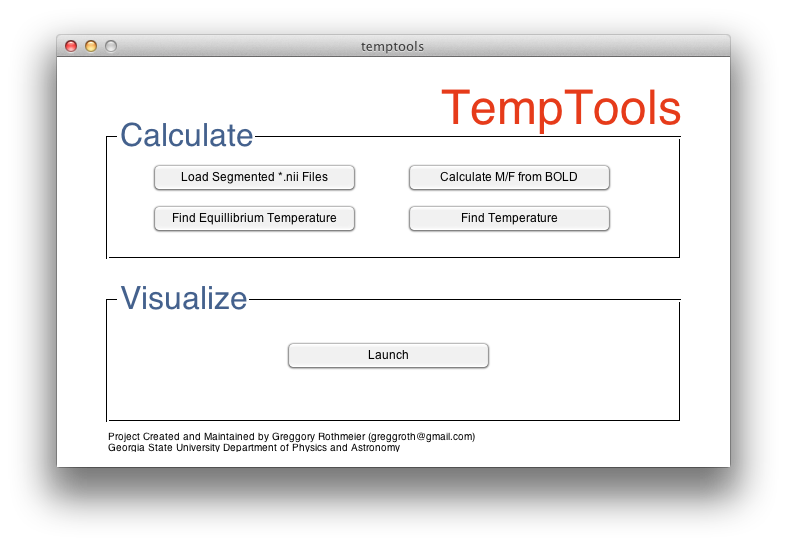
\includegraphics[keepaspectratio=true, width=17cm]{temptools/main.png}
    \caption[temptools: main window]{\label{fig:ttmain} The main window of temptools.  From here, you can go through the calculation steps and launch the visualization tool.}
  \centering
\end{figure}
\begin{figure}[bt]
  \centering
    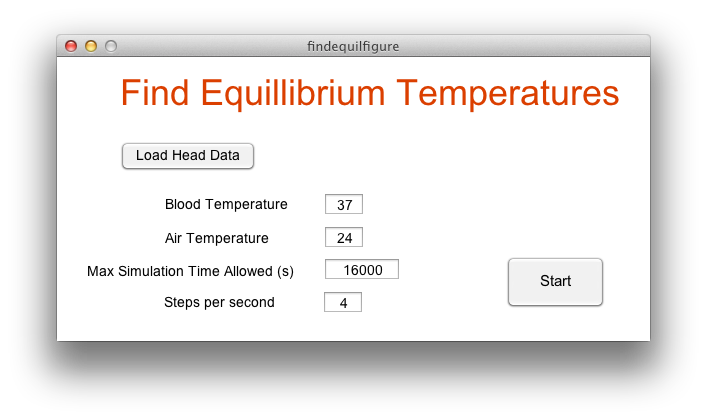
\includegraphics[keepaspectratio=true, width=17cm]{temptools/calcequil}
    \caption[temptools: calculate the equilibrium temperature window]{\label{fig:ttcalcequil} This is the interface for calculating the equilibrium temperature (method explained in~\cref{apdx:findequil}) under certain conditions.}
  \centering
\end{figure}
\begin{figure}[bt]
  \centering
    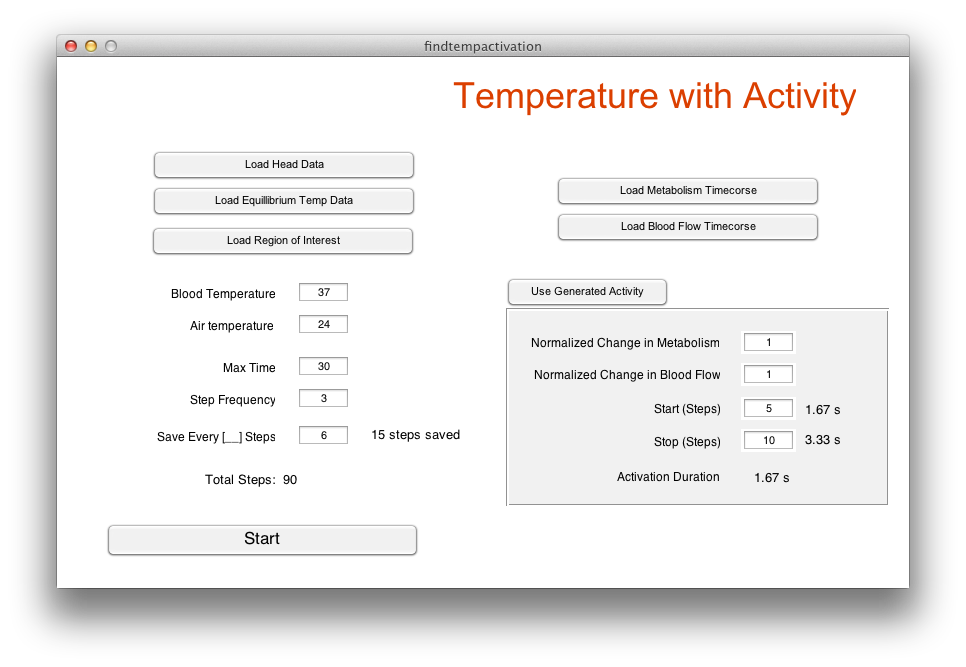
\includegraphics[keepaspectratio=true, width=17cm]{temptools/tempcalc}
    \caption[temptools: calculate temperature during activity]{\label{fig:tttempcalc} The interface for calculating temperature changes when blood flow and metabolism are time dependent.  This can be achieved by either loading metabolism and blood flow datasets or by using generated activity.}
  \centering
\end{figure}
\begin{figure}[bt]
  \centering
    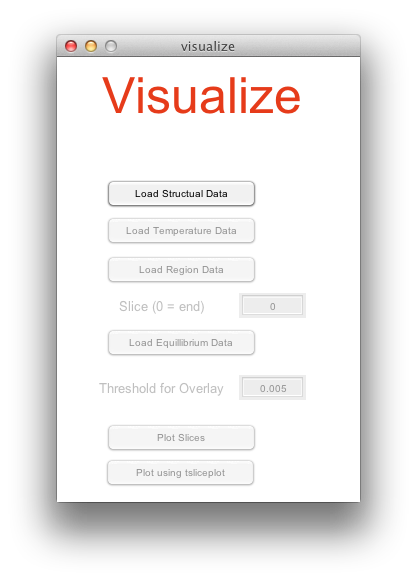
\includegraphics[keepaspectratio=true, width=10cm]{temptools/visualize}
    \caption[temptools: visualize the data]{\label{fig:ttvisualize} Visualize your data using the temptools visualization window.  This loads all of the required data and launches a slice browser or tsliceplot (see \cref{apdx:visualize} for more details).}
  \centering
\end{figure}
% Load T1/create head data
\section{Creating the Head Matrix}
\label{apdx:headmatrix}
Before any calculations can be done, a matrix containing tissue-specific parameters must be created.  First, a T1 contrast image should be segmented using SPM8 (\url{http://www.fil.ion.ucl.ac.uk/spm/software/spm8/}).  For ease of consistency, the one provided by SPM8 in ./canonical/ is best to use.  Using SPM's ``New Segmentation'' algorithim will segment the image into five different tissue types (gray matter, white matter, cerebral spinal fluid, soft tissue and bone).  Once this is complete, run ImportSegmentedT1() within this directory and it will return a matrix that has been populated with the tissue-specific parameters required for accurate temperature calculations. The functions fillAir() (\ref{code:fillair}), fillHoles() (\ref{code:fillHoles}), build\_skin() (\ref{code:buildskin}) and repair\_headdata() (\ref{code:repairheaddata}) are functions required by BulkImportNII().  More information about this procedure is in~\cref{sec:prephead}.
\subsection{ImportSegmentedT1()}
\lstinputlisting[style=codeblock]{code/ImportSegmentedT1.m}
\subsection{fillAir()}
\label{code:fillair}
\lstinputlisting[style=codeblock]{code/fillAir.m}
\subsection{fillHoles()}
\label{code:fillHoles}
\lstinputlisting[style=codeblock]{code/fillHoles.m}
\subsection{build\_skin()}
\label{code:buildskin}
\lstinputlisting[style=codeblock]{"code/build_skin.m"}
\subsection{repair\_headdata()}
\label{code:repairheaddata}
This function will go through the dataset and make sure the tissue-specific parameters are correct for the tissue type assigned for that voxel.  fillAir(), fillHoles() and build\_skin() all correct mislabeled voxels, but they only correct the tissue assignment.  After using any of these functions, the data must be passed through repair\_headdata to update the stored parameters.
\lstinputlisting[style=codeblock]{"code/repair_headdata.m"}
% Load fMRI Data
\clearpage
\section{Loading the fMRI Data}
\label{apdx:fmriprocessing}
The following sections details the processing required to convert the BOLD data (in NIFTI format) to metabolism and blood flow time-courses that can then be used to calculate temperature.
\subsection{sample\_bold\_import()}
The following code automates the procedure of processing and doing all the calculations on the dataset reported in~\citet{dhamala}.  It's is written for my data on my machine, but it can be used to gain a better understanding of the procedure. For a conceptual explanation, see~\cref{sec:calcmf}.
\lstinputlisting[style=codeblock]{"code/sample_bold_import.m"}
\subsection{avg\_NII\_rest()}
\lstinputlisting[style=codeblock]{"code/avg_NII_rest.m"}
\subsection{avg\_NII\_normalize()}
\lstinputlisting[style=codeblock]{"code/avg_NII_normalize.m"}
\subsection{BOLDtoMF()}
\lstinputlisting[style=codeblock]{"code/BOLDtoMF.m"}
\subsection{lambw() and lambw\_mex()}
The lambw() function is a wrapper for the wapr() function available on Matlab FileExchange (\url{http://www.mathworks.com/matlabcentral/fileexchange/3644-real-values-of-the-lambert-w-function/content/Lambert/wapr.m}).  A compiled version of this function (lambw\_mex()) runs much faster and is recommended.  This function is used over Matlab's built-in Lambert-W function for the sake of performance.
\lstinputlisting[style=codeblock]{"code/lambw.m"}
% Find Equilibrium
\clearpage
\section{Calculating the Equilibrium Temperature}
\label{apdx:findequil}
In order to determine the temperature fluctuations due to changes in activity, the baseline temperature must first be established for each voxel.  The function tempCalcEquilibrium() will update the temperature using the Penne's bioheat equation (\cref{eq:3dbioheat}) until the change in temperature for each voxel falls below a certain threshold.  Details about this procedure are available in~\cref{sec:calcequilT}.
\subsection{tempCalcEquilibrium()}
\lstinputlisting[style=codeblock]{code/tempCalcEquilibrium.m}
% Find Temperature Change
\clearpage
\section{Calculating the Temperature Change}
The following function takes as inputs the head data matrix (\cref{apdx:headmatrix}), the metabolism and blood flow time courses (\cref{apdx:fmriprocessing}) and the equilibrium temperatures (\cref{apdx:findequil}) and calculates the temperature time-course.   More details about this algorithm can be found in~\cref{sec:calcT}.
\subsection{tempCalcDynMF}
\label{apdx:tempCalcDynMF}
\lstinputlisting[style=codeblock]{code/tempCalcDynMF.m}
\chapter{Visualization Tools}
\label{apdx:visualize}
The temperature data is a four dimensional dataset (time, x, y and z), so good visualizations tools are necessary to analyzing the results.  The primary tool I use is a modification of SliceBrowser (\url{http://www.mathworks.com/matlabcentral/fileexchange/20604}) and is provided as part of temptools (\url{https://github.com/greggroth/temptools/tree/master/lib/SliceBrowser}).  In working with this, I also created a function (TempPlot()) to act as a wrapper and handle possible plotting situations depending on the number of inputs.
\setcounter{section}{1}
\setcounter{subsection}{0}
\subsection{TempPlot()}
\lstinputlisting[style=codeblock]{code/TempPlot.m}
\subsection{tsliceplot}
This is a visualization tool I wrote that allows you to view the change in temperature versus time for a line passing through the head.  Screenshots of the tool can be seen in~\cref{fig:tsliceplot,fig:tsliceplotz}.

Usage:
\begin{lstlisting}[style=snippet,label=invoke-tsliceplot]
  tsliceplot(temperature_data, equilibrium_temperature_data)
\end{lstlisting}

The script is available as part of temptools (\url{https://github.com/greggroth/temptools/tree/master/lib/tsliceplot}).

\begin{figure}[hbt]
  \centering
    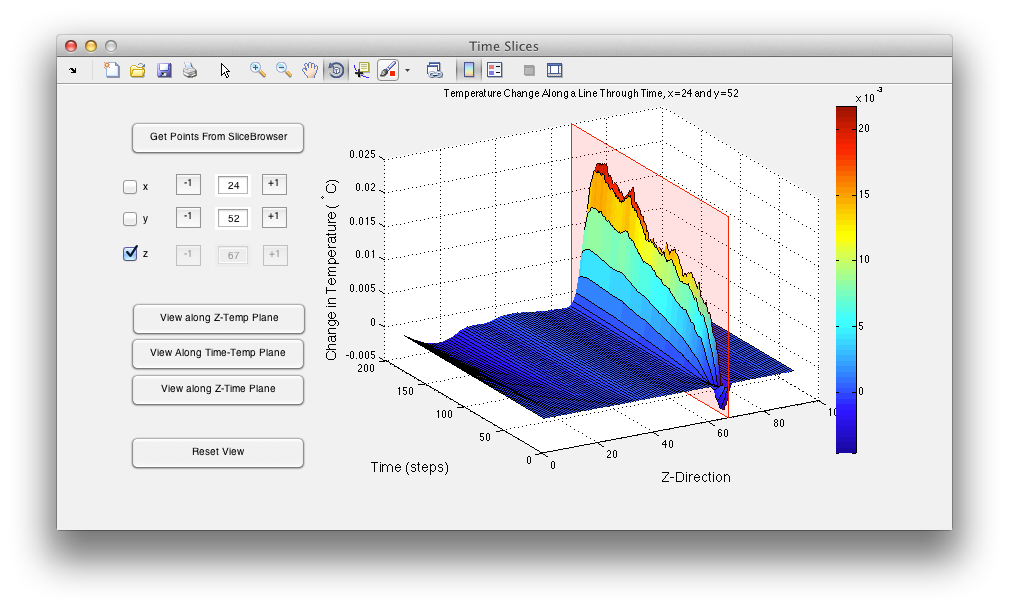
\includegraphics{tsliceplot/default-view}
    \caption[Visualization using tsliceplot]{Experimental data for activity in the motor cortex visualized with tsliceplot. \label{fig:tsliceplot}}
  \centering
\end{figure}

\begin{figure}[hbt]
  \centering
    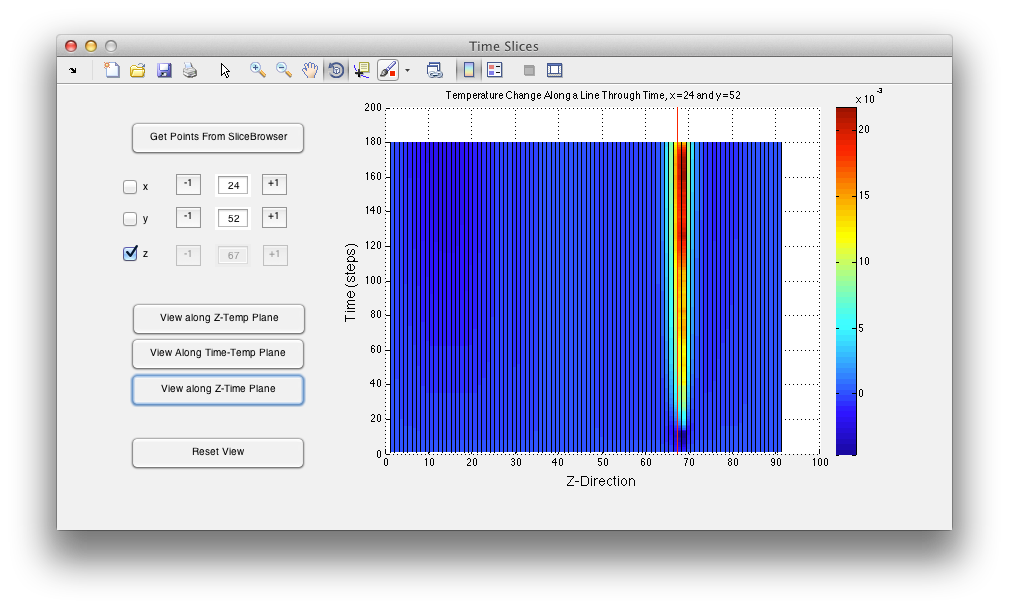
\includegraphics{tsliceplot/z-plane-view}
    \caption[Visualization using tsliceplot (z v. t plane)]{The same data as is presented in~\cref{fig:tsliceplot}, but viewed flat-on along the z vs. time plane.\label{fig:tsliceplotz}}
  \centering
\end{figure}
  
\end{document}